
\chapter{Analysis by Cover Type}
\label{ch:covtype}
We defined 31 distinct land cover types in the Yuba River watershed and surrounding area for the purposes of \textsc{RMLands} simulations (Table~\ref{covertable}). A few of these were located in the buffer, but not the project area. Several others were treated as \emph{static} in the simulation: they did not undergo vegetation transitions over time or in response to fire. However, four of the \emph{static} types were allowed to experience wildfires: Agriculture, Grassland, Meadow, and Urban. Grasslands may experience fire, but because they are expected to recover from fire in less than five years (the length of one timestep in our simulation), we assume they remain constant in composition and structure. The discussion that follows focuses on the nine cover types found within the core project area that were treated as dynamic in the model and that occurred over an extent of at least 1000 ha in the project area. For each of these cover types, we briefly describe the simulated disturbance regime (i.e., spatial extent and distribution, frequency and temporal variability) associated with each relevant disturbance process, the vegetation dynamics resulting from the interplay between these disturbance processes and succession, and an examination of the cover type’s current departure from the simulated HRV. 

%\subsection{Curl-leaf Mountain Mahogany}
%\subsection{Lodgepole Pine} 
%\subsection{Lodgepole Pine with Aspen}
%\subsection{Mixed Evergreen - Ultramafic} 
%\subsection{Montane Riparian} 
%\subsection{Oak Woodland} 
%\subsection{Red Fir - Ultramafic} 
%\subsection{Red Fir with Aspen} 
%\subsection{Sierran Mixed Conifer with Aspen} 
%\subsection{Subalpine Conifer} 
%\subsection{Western White Pine} 


%topics
% CHECK disturbed area
% climate? tpi? - Looked at climate for OCFW...basically the same as for landscape. not sure what it adds

%%%%%%%%%%%%%%%%%%%%%%%%%%%%%%%%%%%%%%%%%%%%%%%%%%%%%%%%%%%%%%%%%%%%%%%%%%%%%
%%%%%%%%%%%%%%%%%%%%%%%%%%%%%%%%%%%%%%%%%%%%%%%%%%%%%%%%%%%%%%%%%%%%%%%%%%%%%
%%%%%%%%%%%%%%%%%%%%%%%%%%%%%%%%%%%%%%%%%%%%%%%%%%%%%%%%%%%%%%%%%%%%%%%%%%%%%
%%%%%%%%%%%%%%%%%%%%%%%%%%%%%%%%%%%%%%%%%%%%%%%%%%%%%%%%%%%%%%%%%%%%%%%%%%%%%
%%%%%%%%%%%%%%%%%%%%%%%%%%%%%%%%%%%%%%%%%%%%%%%%%%%%%%%%%%%%%%%%%%%%%%%%%%%%%
\section{Notes on repairing error}
Fixed darea-covertype plots and darea-hist-covertype plots. Fixed darea tables. In the long run, reorganize so that cover types appear in order of importance/area.
Updated darea, preturn comments.
Updated covcond comments.
Updated TPI
Updated fragclass results

To update
fragclass results

%\clearpage
\section{Mixed Evergreen - Mesic} 

\begin{figure}[!htbp]
  \centering
  \subfloat[][]{
    \centering
    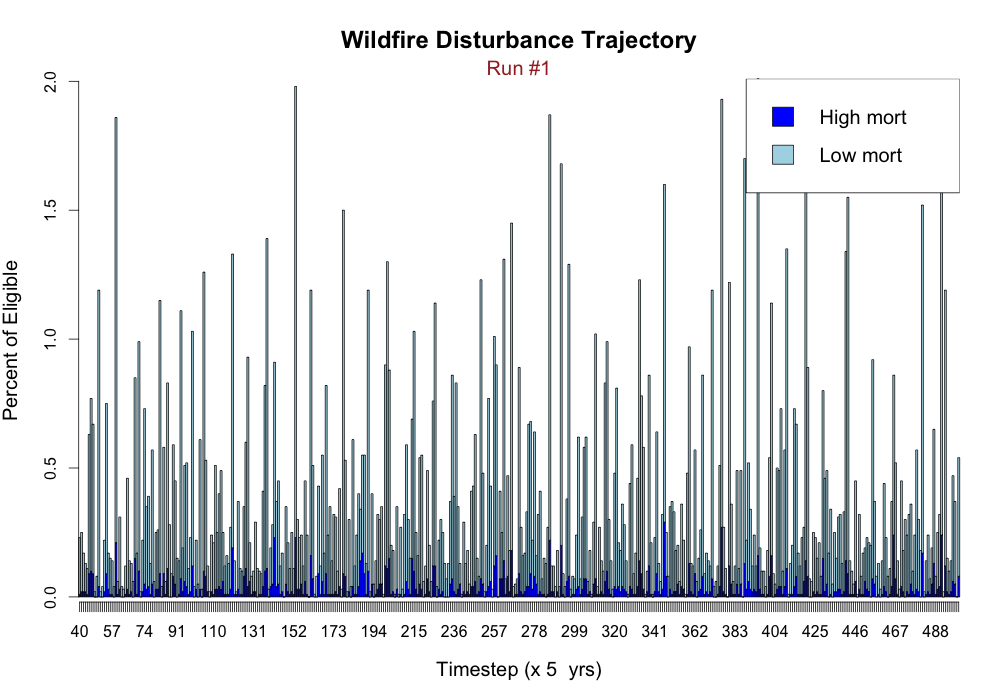
\includegraphics[width=0.5\textwidth]{/Users/mmallek/Tahoe/Report2/images/darea_megm.png}
    }%
  \subfloat[][]{
    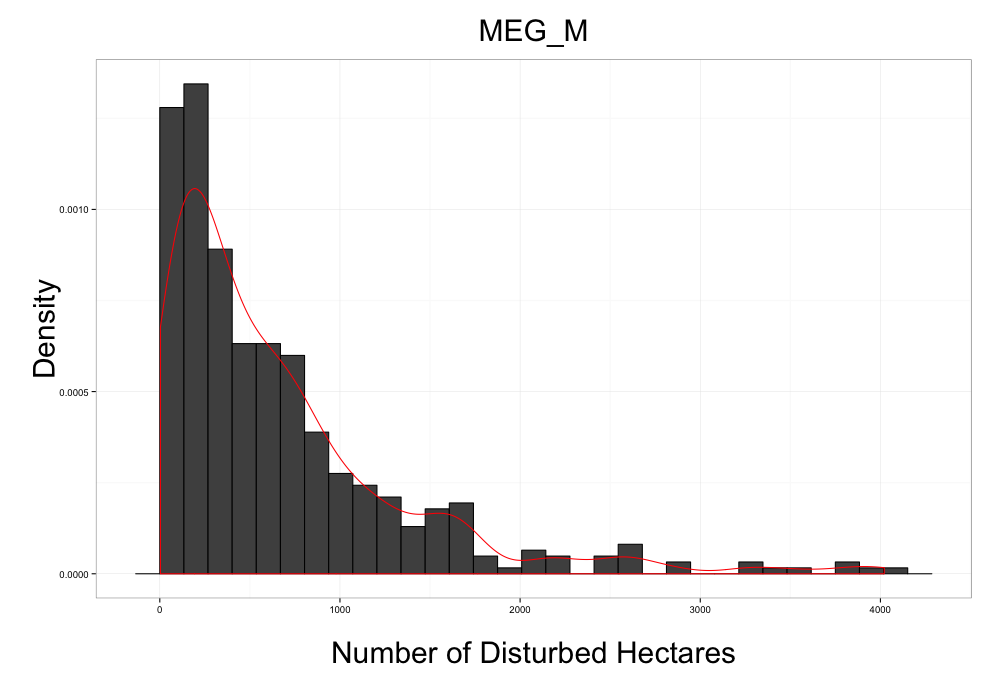
\includegraphics[width=0.5\textwidth]{/Users/mmallek/Tahoe/Report2/images/darea_hist_megm.png}
    }
  \caption{(a) \small Disturbance trajectory for Mixed Evergreen - Mesic. High mortality fire in dark blue; low mortality fire in light blue. (b) Histogram of disturbed hectares with density curve overlaid.} 
  \label{fig:darea_megm}
\end{figure}

Mixed Evergreen - Mesic (\textsc{meg\_m}) is a somewhat common cover type within the core project area, encompassing 7,273 ha and comprising roughly 4\% of the project area. The frequency and extent of simulated wildfires in mesic mixed evergreen forest varied markedly across the landscape (Figure~\ref{fig:darea_megm} and Table~\ref{tab:darea_megm}). %
%
While mesic mixed evergreen forests always experienced some wildfire during the simulation, during a typical five year period wildfires burned a small portion of the cover type, but the impacts were mostly low mortality. Low mortality fires were eight times as frequent as high mortality fires. Less than 1\% of the cover type (72 ha) burned during 9\% of the timesteps. Much more common were timesteps in which over 10\% of the landscape burned, which occurred about once in 17 years. The median proportion burned was 6\%. Seldom did large extents burn, at any mortality level, although roughly once every 68 years, more than 25\% of the cover type burned. We never observed a timestep during which more than 50\% of these forests experienced wildfire. The maximum extent burned within the cover type was about 48\% (about 3,500 ha). %
%
Under this wildfire regime, the grand mean return interval between fires (of any mortality level) varied widely from 19 years to more than 500 years, with a median of 62 years (Figure~\ref{fig:preturn_megm}). The median return interval and rotation values were influenced primarily by the dominant fire type, low mortality. Mesic mixed evergreen forests had a low mortality fire rotation of 63 years and a high mortality fire rotation of 534 years. %
\begin{table}[!htbp]
\centering
\caption{\small Disturbed area summary statistics for Mixed Evergreen - Mesic. Proportions shown are relative to the total area of Mixed Evergreen - Mesic.}
\label{tab:darea_megm}
  \begin{tabular}{@{}llll@{}} 
  \toprule
  \textbf{\begin{tabular}[c]{@{}l@{}}Summary Statistic \\ (disturbed area/timestep)\end{tabular}} & \textbf{\begin{tabular}[c]{@{}l@{}}Low  Mortality\end{tabular}} & \textbf{\begin{tabular}[c]{@{}l@{}}High  Mortality\end{tabular}} & \textbf{\begin{tabular}[c]{@{}l@{}}Any  Mortality\end{tabular}} \\ \midrule
  Minimum       & 0.05  & 0.00 & 0.05  \\
  Maximum       & 49.36 & 8.66 & 55.29 \\
  Median        & 5.44  & 0.57 & 6.11  \\
  Mean          & 8.11  & 0.95 & 9.10  \\
  \textbf{Fire Rotation}  & 61       & 525       & 55 \\  \bottomrule
  \end{tabular}
\end{table}
%
In general, return intervals and canopy cover varied spatially across the forest and increased slightly with increasing TPI, an unexpected result. This is likely related to the fact that during the simulated HRV, the vast majority of these stands were in closed canopy conditions, regardless of topographic position. Canopy cover increased by about 1.5\% when comparing minimum to maximum TPI (Table~\ref{tab:tpi_cc}). %
%
Finally, when stands of mesic mixed evergreen forests were adjacent to cover types with shorter return intervals, they also exhibited shorter return intervals, reflecting the importance of landscape context on fire regimes.

%%%
The age structure and dynamics of mesic mixed evergreen forest illustrates the interaction between disturbance and succession processes. We focus our analysis on the 5$^{\text{th}}$ to 95$^{\text{th}}$ percentile range of variability for our simulation (excluding the equilibration period). %
%
The distribution of area among stand conditions within mesic mixed evergreen forest fluctuated over time (Figure~\ref{fig:covcond_megm}). Because high mortality fire is very rare in this cover type, and the time to reaching a Late Development stage is relatively short (Appendix \ref{sec:covertypedesc}), the vast majority of the landscape, varying from 71\% to 88\%, was in the Late Development - Closed condition during the simulation (Table~\ref{tab:covcond1}). %
%
The seral-stage distribution appeared to be in dynamic equilibrium (i.e., the percentage in each stand condition varied about a stable mean). Our calculated current seral-stage distribution was never observed under the simulated HRV (Table~\ref{tab:covcond1}, Figure~\ref{fig:covcondbar_megm}). The most notable departure was the shift from Mid Development to Late Development condition classes. About 52\% of the current landscape is comprised of the mesic mixed evergreen forest in mid development conditions, but the late development conditions were always dominant under the simulated HRV. The current proportions of all mid development canopy cover levels are higher than at any point during the HRV. As described above, much of the shift from the dominance of mid development conditions observed in the current distribution to the dominance by late development conditions during the HRV can be attributed to the prodigious increase in the extent of Late Development - Closed (from 29\% to 71-88\%), although Late Development - Moderate was also well represented, with an HRV from 6\%--15\%. The Early Development condition is also more common on the current landscape than during the simulation.


\begin{figure}[!htbp]
  %\centering
  \subfloat[][]{
%    \centering
    \includegraphics[width=0.8\textwidth]{/Users/mmallek/Tahoe/Report2/images/CovcondHRVBarplots/megm_Early-AllStructures_srvplot_.pdf}
  }\\%
  \subfloat[][]{
%    \centering
    \includegraphics[width=0.8\textwidth]{/Users/mmallek/Tahoe/Report2/images/CovcondHRVBarplots_nolegend/megm_Mid-Closed_srvplot_.pdf}
  }\\%
    \subfloat[][]{
%    \centering
    \includegraphics[width=0.8\textwidth]{/Users/mmallek/Tahoe/Report2/images/CovcondHRVBarplots_nolegend/megm_Mid-Moderate_srvplot_.pdf}
  }\\%
    \subfloat[][]{
%    \centering
    \includegraphics[width=0.8\textwidth]{/Users/mmallek/Tahoe/Report2/images/CovcondHRVBarplots_nolegend/megm_Mid-Open_srvplot_.pdf}
  }\\%
    \subfloat[][]{
%    \centering
    \includegraphics[width=0.8\textwidth]{/Users/mmallek/Tahoe/Report2/images/CovcondHRVBarplots_nolegend/megm_Late-Closed_srvplot_.pdf}
  }\\%
    \subfloat[][]{
%    \centering
    \includegraphics[width=0.8\textwidth]{/Users/mmallek/Tahoe/Report2/images/CovcondHRVBarplots_nolegend/megm_Late-Moderate_srvplot_.pdf}
  }\\%
    \subfloat[][]{
%    \centering
    \includegraphics[width=0.8\textwidth]{/Users/mmallek/Tahoe/Report2/images/CovcondHRVBarplots_nolegend/megm_Late-Open_srvplot_.pdf}
  }\\%
  \caption{Cover-condition barplots for Mixed Evergreen - Mesic dynamics. For each condition class, the color the bar represents the distance from the median value during the simulated HRV. Green represents the 25th-75th percentiles; yellow represents the 5th-25th and 75th to 95th percentiles; red represents the 0th-5th and 95th-100th percentiles. The blue vertical line marks the 50th percentile and the black vertical line indicates the current cover extent. To read the ``Early–All Structures'' barplot, for a given percentage of the cover type extent, the x-axis value indicates an observed proportion, and the color corresponding to that point indicates the percentile range that value falls within. In this example, the current percent of cover extent for this cover type and condition class falls within the 95th-100th percentile range during the simulated HRV.}
  \label{fig:covcondbar_megm}
\end{figure}

The spatial configuration of stand conditions fluctuated markedly over time as well, although there was considerable variation in the magnitude of variability among configuration metrics (Appendix \ref{sec:full-class-results}). Area-weighted patch and core area, edge density, and patch density exhibited the greatest variability over time. Because the landscape is so dominated by the Late Development - Closed and Moderate conditions, we focus on the configuration metrics for these classes. In general, the current landscape contains fewer, smaller, and more clumped patches than existed under the simulated HRV. Current patches in Late Development - Closed are less geometrically complex and have less area in cores than during the simulated HRV.


\begin{figure}[!htbp]
  \subfloat[][]{
    \includegraphics[width=0.8\textwidth]{/Users/mmallek/Tahoe/Report2/images/ClassFragPlots_wlegend/AREA_AM-MEG_M_EARLY_ALL-srvplot-.pdf}
  }\\%
  \subfloat[][]{
    \includegraphics[width=0.8\textwidth]{/Users/mmallek/Tahoe/Report2/images/ClassFragPlots_nolegend/AREA_AM-MEG_M_MID_CL-srvplot-.pdf}
  }\\%
    \subfloat[][]{

    \includegraphics[width=0.8\textwidth]{/Users/mmallek/Tahoe/Report2/images/ClassFragPlots_nolegend/AREA_AM-MEG_M_MID_MOD-srvplot-.pdf}
  }\\%
    \subfloat[][]{
    \includegraphics[width=0.8\textwidth]{/Users/mmallek/Tahoe/Report2/images/ClassFragPlots_nolegend/AREA_AM-MEG_M_MID_OP-srvplot-.pdf}
  }\\%
    \subfloat[][]{
    \includegraphics[width=0.8\textwidth]{/Users/mmallek/Tahoe/Report2/images/ClassFragPlots_nolegend/AREA_AM-MEG_M_LATE_CL-srvplot-.pdf}
  }\\%
    \subfloat[][]{
    \includegraphics[width=0.8\textwidth]{/Users/mmallek/Tahoe/Report2/images/ClassFragPlots_nolegend/AREA_AM-MEG_M_LATE_MOD-srvplot-.pdf}
  }\\%
    \subfloat[][]{
%    \centering
    \includegraphics[width=0.8\textwidth]{/Users/mmallek/Tahoe/Report2/images/ClassFragPlots_nolegend/AREA_AM-MEG_M_LATE_OP-srvplot-.pdf}
  }\\%
  \caption{Fragstats class-level results for Mixed Evergreen - Mesic and area-weighted mean patch area. Each bar denotes the metric value for the associated percentile value. A blue bar denotes the median simulated HRV value and a black bar denotes the current value.}
  \label{fig:megm_areaam}
\end{figure}

\begin{figure}[!htbp]
  \subfloat[][]{
    \includegraphics[width=0.8\textwidth]{/Users/mmallek/Tahoe/Report2/images/ClassFragPlots_wlegend/CORE_AM-MEG_M_EARLY_ALL-srvplot-.pdf}
  }\\%
  \subfloat[][]{
    \includegraphics[width=0.8\textwidth]{/Users/mmallek/Tahoe/Report2/images/ClassFragPlots_nolegend/CORE_AM-MEG_M_MID_CL-srvplot-.pdf}
  }\\%
    \subfloat[][]{

    \includegraphics[width=0.8\textwidth]{/Users/mmallek/Tahoe/Report2/images/ClassFragPlots_nolegend/CORE_AM-MEG_M_MID_MOD-srvplot-.pdf}
  }\\%
    \subfloat[][]{
    \includegraphics[width=0.8\textwidth]{/Users/mmallek/Tahoe/Report2/images/ClassFragPlots_nolegend/CORE_AM-MEG_M_MID_OP-srvplot-.pdf}
  }\\%
    \subfloat[][]{
    \includegraphics[width=0.8\textwidth]{/Users/mmallek/Tahoe/Report2/images/ClassFragPlots_nolegend/CORE_AM-MEG_M_LATE_CL-srvplot-.pdf}
  }\\%
    \subfloat[][]{
    \includegraphics[width=0.8\textwidth]{/Users/mmallek/Tahoe/Report2/images/ClassFragPlots_nolegend/CORE_AM-MEG_M_LATE_MOD-srvplot-.pdf}
  }\\%
    \subfloat[][]{
%    \centering
    \includegraphics[width=0.8\textwidth]{/Users/mmallek/Tahoe/Report2/images/ClassFragPlots_nolegend/CORE_AM-MEG_M_LATE_OP-srvplot-.pdf}
  }\\%
  \caption{Fragstats class-level results for Mixed Evergreen - Mesic and area-weighted mean patch core area. Each bar denotes the metric value for the associated percentile value. A blue bar denotes the median simulated HRV value and a black bar denotes the current value.}
  \label{fig:megm_coream}
\end{figure}



\begin{figure}[!htbp]
  \subfloat[][]{
    \includegraphics[width=0.8\textwidth]{/Users/mmallek/Tahoe/Report2/images/ClassFragPlots_wlegend/SHAPE_AM-MEG_M_EARLY_ALL-srvplot-.pdf}
  }\\%
  \subfloat[][]{
    \includegraphics[width=0.8\textwidth]{/Users/mmallek/Tahoe/Report2/images/ClassFragPlots_nolegend/SHAPE_AM-MEG_M_MID_CL-srvplot-.pdf}
  }\\%
    \subfloat[][]{

    \includegraphics[width=0.8\textwidth]{/Users/mmallek/Tahoe/Report2/images/ClassFragPlots_nolegend/SHAPE_AM-MEG_M_MID_MOD-srvplot-.pdf}
  }\\%
    \subfloat[][]{
    \includegraphics[width=0.8\textwidth]{/Users/mmallek/Tahoe/Report2/images/ClassFragPlots_nolegend/SHAPE_AM-MEG_M_MID_OP-srvplot-.pdf}
  }\\%
    \subfloat[][]{
    \includegraphics[width=0.8\textwidth]{/Users/mmallek/Tahoe/Report2/images/ClassFragPlots_nolegend/SHAPE_AM-MEG_M_LATE_CL-srvplot-.pdf}
  }\\%
    \subfloat[][]{
    \includegraphics[width=0.8\textwidth]{/Users/mmallek/Tahoe/Report2/images/ClassFragPlots_nolegend/SHAPE_AM-MEG_M_LATE_MOD-srvplot-.pdf}
  }\\%
    \subfloat[][]{
%    \centering
    \includegraphics[width=0.8\textwidth]{/Users/mmallek/Tahoe/Report2/images/ClassFragPlots_nolegend/SHAPE_AM-MEG_M_LATE_OP-srvplot-.pdf}
  }\\%
  \caption{Fragstats class-level results for Mixed Evergreen - Mesic and area-weighted mean patch shape. Each bar denotes the metric value for the associated percentile value. A blue bar denotes the median simulated HRV value and a black bar denotes the current value.}
  \label{fig:megm_shapeam}
\end{figure}

\begin{figure}[!htbp]
  \subfloat[][]{
    \includegraphics[width=0.8\textwidth]{/Users/mmallek/Tahoe/Report2/images/ClassFragPlots_wlegend/CLUMPY-MEG_M_EARLY_ALL-srvplot-.pdf}
  }\\%
  \subfloat[][]{
    \includegraphics[width=0.8\textwidth]{/Users/mmallek/Tahoe/Report2/images/ClassFragPlots_nolegend/CLUMPY-MEG_M_MID_CL-srvplot-.pdf}
  }\\%
    \subfloat[][]{

    \includegraphics[width=0.8\textwidth]{/Users/mmallek/Tahoe/Report2/images/ClassFragPlots_nolegend/CLUMPY-MEG_M_MID_MOD-srvplot-.pdf}
  }\\%
    \subfloat[][]{
    \includegraphics[width=0.8\textwidth]{/Users/mmallek/Tahoe/Report2/images/ClassFragPlots_nolegend/CLUMPY-MEG_M_MID_OP-srvplot-.pdf}
  }\\%
    \subfloat[][]{
    \includegraphics[width=0.8\textwidth]{/Users/mmallek/Tahoe/Report2/images/ClassFragPlots_nolegend/CLUMPY-MEG_M_LATE_CL-srvplot-.pdf}
  }\\%
    \subfloat[][]{
    \includegraphics[width=0.8\textwidth]{/Users/mmallek/Tahoe/Report2/images/ClassFragPlots_nolegend/CLUMPY-MEG_M_LATE_MOD-srvplot-.pdf}
  }\\%
    \subfloat[][]{
%    \centering
    \includegraphics[width=0.8\textwidth]{/Users/mmallek/Tahoe/Report2/images/ClassFragPlots_nolegend/CLUMPY-MEG_M_LATE_OP-srvplot-.pdf}
  }\\%
  \caption{Fragstats class-level results for Mixed Evergreen - Mesic and clumpiness. Each bar denotes the metric value for the associated percentile value. A blue bar denotes the median simulated HRV value and a black bar denotes the current value.}
  \label{fig:megm_clumpy}
\end{figure}

%%%%%%%%%%%%%%%%%%%%%%%%%%%%%%%%%%%%%%%%%%%%%%%%%%%%%%%%%%%%%%%%%%%%%%%%%%%%%
%%%%%%%%%%%%%%%%%%%%%%%%%%%%%%%%%%%%%%%%%%%%%%%%%%%%%%%%%%%%%%%%%%%%%%%%%%%%%
%%%%%%%%%%%%%%%%%%%%%%%%%%%%%%%%%%%%%%%%%%%%%%%%%%%%%%%%%%%%%%%%%%%%%%%%%%%%%
%%%%%%%%%%%%%%%%%%%%%%%%%%%%%%%%%%%%%%%%%%%%%%%%%%%%%%%%%%%%%%%%%%%%%%%%%%%%%
%%%%%%%%%%%%%%%%%%%%%%%%%%%%%%%%%%%%%%%%%%%%%%%%%%%%%%%%%%%%%%%%%%%%%%%%%%%%%

\clearpage
\section{Mixed Evergreen - Xeric} 

\begin{figure}[!htbp]
  \centering
  \subfloat[][]{
    \centering
    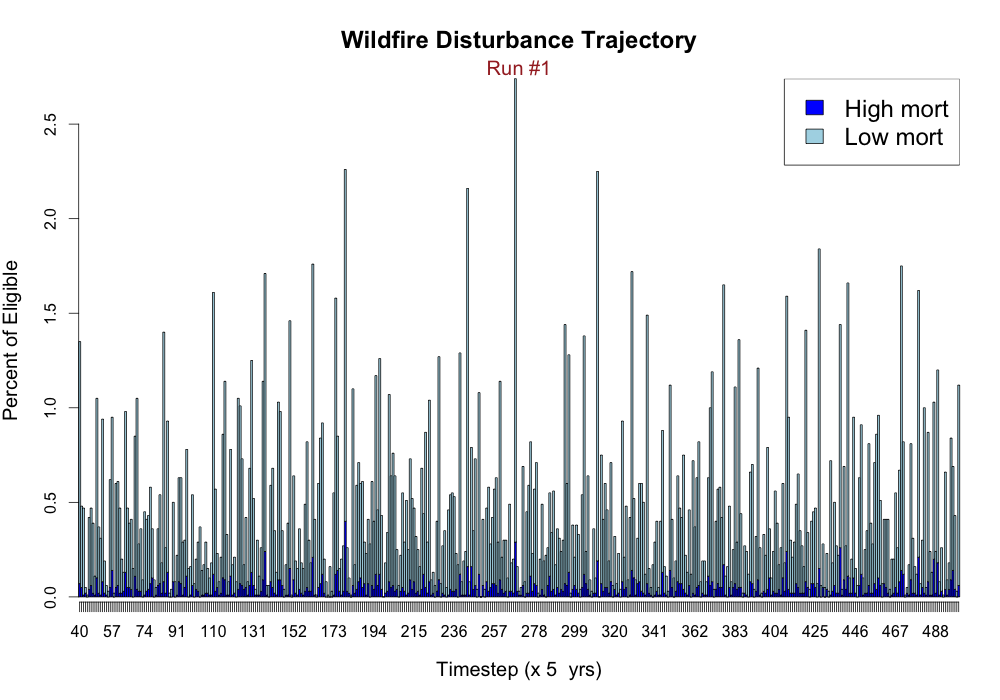
\includegraphics[width=0.5\textwidth]{/Users/mmallek/Tahoe/Report2/images/darea_megx.png}
    }%
  \subfloat[][]{
    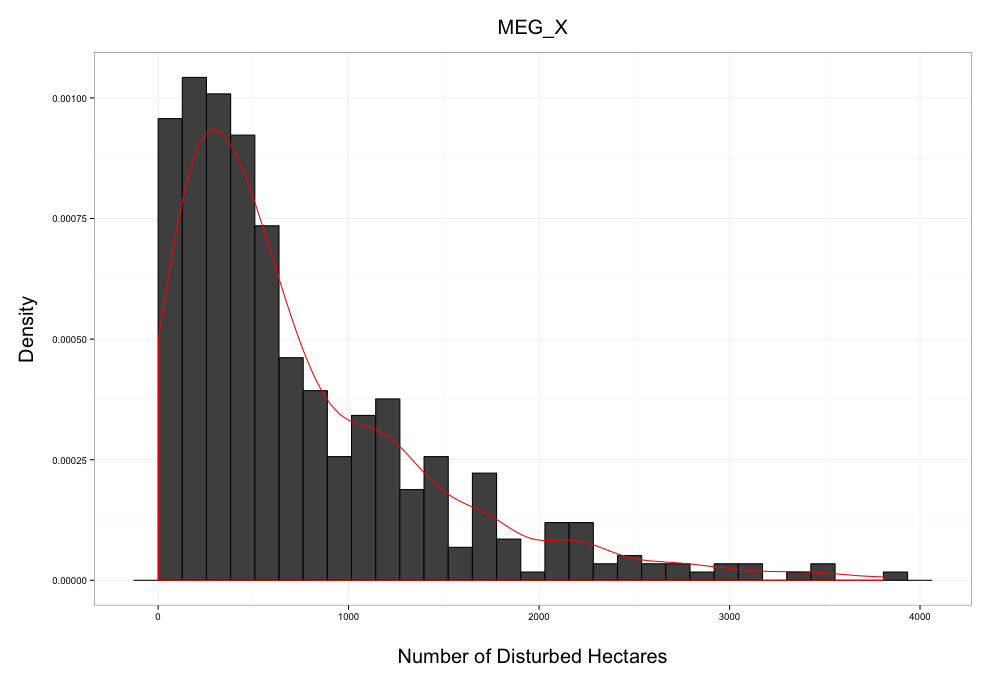
\includegraphics[width=0.5\textwidth]{/Users/mmallek/Tahoe/Report2/images/darea_hist_megx.png}
    }
  \caption{\small (a) Disturbance trajectory for Mixed Evergreen - Xeric. High mortality fire in dark blue; low mortality fire in light blue. (b) Histogram of disturbed hectares with density curve overlaid.} 
  \label{fig:darea_megx}
\end{figure}


Mixed Evergreen - Xeric (\textsc{meg\_x})is a somewhat common cover type within the core project area, encompassing 6,768 ha and comprising roughly 4\% of the project area. The frequency and extent of simulated wildfires in xeric mixed evergreen forest varied markedly across the landscape (Figure~\ref{fig:darea_megx} and Table~\ref{tab:darea_megx}). %
%
While xeric mixed evergreen forests always experienced some wildfire during the simulation, during a typical five year period wildfires burned across a larger extent on average than the mesic mixed evergreen forest, but the impacts were mostly low mortality. Low mortality fires were several times more frequent as high mortality fires, although proportions varied widely across timesteps. At least some area burned every timestep. Timesteps in which over 10\% of the landscape burned occurred about once in 13 years. The median proportion burned was 8\%. Seldom did large extents burn, at any mortality level, although roughly once every 46 years, more than 25\% of the cover type burned. Over 50\% of the landscape on very rare occasions (once in about 770 years). The maximum extent burned within the cover type was about 56\% (about 3,800 ha). %
%
Under this wildfire regime, the return interval between fires (of any mortality level) varied widely from 19 years to over 500 years, with a median of 45 years (Figure~\ref{fig:preturn_megm}). The median return interval and rotation values were influenced primarily by the dominant fire type, low mortality. Xeric mixed evergreen forests had a low mortality fire rotation of 47 years and a high mortality fire rotation of 434 years (Table~\ref{tab:darea_megm}).  %
%
In general, return intervals and canopy cover varied spatially across the forest and increased slightly with increasing TPI, an unexpected result. This is likely related to the fact that during the simulated HRV, the vast majority of these stands were in closed canopy conditions, regardless of topographic position. Canopy cover increased by about 3.8\% when comparing minimum to maximum TPI (Table~\ref{tab:tpi_cc}). %
%
Finally, when stands of xeric mixed evergreen forests were adjacent to cover types with shorter return intervals, they also exhibited shorter return intervals, reflecting the importance of landscape context on fire regimes.

\begin{table}[!htbp]
\centering
\caption{\small Disturbed area summary statistics for Mixed Evergreen - Xeric. Proportions shown are relative to the total area of Mixed Evergreen - Xeric.}
\label{tab:darea_megx}
\begin{tabular}{@{}llll@{}}
\toprule
\textbf{\begin{tabular}[c]{@{}l@{}}Summary Statistic \\ (disturbed area/timestep)\end{tabular}} & \textbf{Low Mortality} & \textbf{High Mortality} & \textbf{Any Mortality} \\ \midrule
Minimum       & 0.10  & 0.00  & 0.10  \\ 
Maximum       & 63.26 & 10.21 & 70.67 \\ 
Median        & 7.70  & 0.75  & 8.81  \\ 
Mean          & 10.62 & 1.15  & 11.83 \\
\textbf{Fire Rotation}  & 47       & 434       & 42 \\ \bottomrule
\end{tabular}
\end{table}


%%%
The age structure and dynamics of xeric mixed evergreen forest illustrates the interaction between disturbance and succession processes. We focus our analysis on the 5$^{\text{th}}$ to 95$^{\text{th}}$ percentile range of variability for our simulation (excluding the equilibration period). %
%
The distribution of area among stand conditions within xeric mixed evergreen forest fluctuated over time (Figure~\ref{fig:covcond_megx}). Because high mortality fire is very rare in this cover type, and the time to reaching a Late Development stage is relatively short (Appendix~\ref{sec:covertypedesc}), the vast majority of the landscape, varying from 55\% to 80\%, was in the Late Development - Closed condition during the simulation (Table~\ref{tab:covcond1}).  %
%
The seral-stage distribution appeared to be in dynamic equilibrium (i.e., the percentage in each stand condition varied about a stable mean). Our calculated current seral-stage distribution was never observed under the simulated HRV (Table~\ref{tab:covcond1}). The most notable departure was the shift from Early and Mid Development to Late Development conditions. The current landscape contains 71\% of the xeric mixed evergreen forest in mid development conditions, but the late development conditions were always dominant under the simulated HRV. The current proportions of all mid development canopy cover levels are higher than at any point during the HRV. As described above, much of the shift from the dominance of mid development conditions observed in the current distribution to the dominance by late development conditions during the HRV can be attributed to the prodigious increase in the extent of Late Development - Closed (from 13\% to 55-80\%), although Late Development - Moderate was also well represented, with an HRV from 6\% to 15\%. The Early Development condition is also more common on the current landscape than during the simulation.

\begin{figure}[!htbp]
  %\centering
  \subfloat[][]{
%    \centering
    \includegraphics[width=0.8\textwidth]{/Users/mmallek/Tahoe/Report2/images/CovcondHRVBarplots/megx_Early-AllStructures_srvplot_.pdf}
  }\\%
  \subfloat[][]{
%    \centering
    \includegraphics[width=0.8\textwidth]{/Users/mmallek/Tahoe/Report2/images/CovcondHRVBarplots_nolegend/megx_Mid-Closed_srvplot_.pdf}
  }\\%
    \subfloat[][]{
%    \centering
    \includegraphics[width=0.8\textwidth]{/Users/mmallek/Tahoe/Report2/images/CovcondHRVBarplots_nolegend/megx_Mid-Moderate_srvplot_.pdf}
  }\\%
    \subfloat[][]{
%    \centering
    \includegraphics[width=0.8\textwidth]{/Users/mmallek/Tahoe/Report2/images/CovcondHRVBarplots_nolegend/megx_Mid-Open_srvplot_.pdf}
  }\\%
    \subfloat[][]{
%    \centering
    \includegraphics[width=0.8\textwidth]{/Users/mmallek/Tahoe/Report2/images/CovcondHRVBarplots_nolegend/megx_Late-Closed_srvplot_.pdf}
  }\\%
    \subfloat[][]{
%    \centering
    \includegraphics[width=0.8\textwidth]{/Users/mmallek/Tahoe/Report2/images/CovcondHRVBarplots_nolegend/megx_Late-Moderate_srvplot_.pdf}
  }\\%
    \subfloat[][]{
%    \centering
    \includegraphics[width=0.8\textwidth]{/Users/mmallek/Tahoe/Report2/images/CovcondHRVBarplots_nolegend/megx_Late-Open_srvplot_.pdf}
  }\\%
  \caption{Cover-condition barplots for Mixed Evergreen - Xeric dynamics. For each condition class, the color the bar represents the distance from the median value during the simulated HRV. Green represents the 25th-75th percentiles; yellow represents the 5th-25th and 75th to 95th percentiles; red represents the 0th-5th and 95th-100th percentiles. The blue vertical line marks the 50th percentile and the black vertical line indicates the current cover extent. To read the ``Early–All Structures'' barplot, for a given percentage of the cover type extent, the x-axis value indicates an observed proportion, and the color corresponding to that point indicates the percentile range that value falls within. In this example, the current percent of cover extent for this cover type and condition class falls within the 95th-100th percentile range during the simulated HRV.}
  \label{fig:covcondbar_megx}
\end{figure}

The spatial configuration of stand conditions fluctuated markedly over time as well, although there was considerable variation in the magnitude of variability among configuration metrics (Appendix \ref{sec:full-class-results}). Area-weighted patch and core area, patch density, and radius of gyration exhibited the greatest variability over time. Because the landscape is so dominated by the late development, closed canopy cover condition, we use its configuration metrics as a proxy for the cover tyep as a whole. In general, the current landscape contains fewer, smaller, and more isolated patches than existed under the simulated HRV. Patches in Late Development - Closed are less geometrically complex and have less area in cores in the current landscape than during the simulated HRV. 

\begin{figure}[!htbp]
  \subfloat[][]{
    \includegraphics[width=0.8\textwidth]{/Users/mmallek/Tahoe/Report2/images/ClassFragPlots_wlegend/AREA_AM-MEG_X_EARLY_ALL-srvplot-.pdf}
  }\\%
  \subfloat[][]{
    \includegraphics[width=0.8\textwidth]{/Users/mmallek/Tahoe/Report2/images/ClassFragPlots_nolegend/AREA_AM-MEG_X_MID_CL-srvplot-.pdf}
  }\\%
    \subfloat[][]{

    \includegraphics[width=0.8\textwidth]{/Users/mmallek/Tahoe/Report2/images/ClassFragPlots_nolegend/AREA_AM-MEG_X_MID_MOD-srvplot-.pdf}
  }\\%
    \subfloat[][]{
    \includegraphics[width=0.8\textwidth]{/Users/mmallek/Tahoe/Report2/images/ClassFragPlots_nolegend/AREA_AM-MEG_X_MID_OP-srvplot-.pdf}
  }\\%
    \subfloat[][]{
    \includegraphics[width=0.8\textwidth]{/Users/mmallek/Tahoe/Report2/images/ClassFragPlots_nolegend/AREA_AM-MEG_X_LATE_CL-srvplot-.pdf}
  }\\%
    \subfloat[][]{
    \includegraphics[width=0.8\textwidth]{/Users/mmallek/Tahoe/Report2/images/ClassFragPlots_nolegend/AREA_AM-MEG_X_LATE_MOD-srvplot-.pdf}
  }\\%
    \subfloat[][]{
%    \centering
    \includegraphics[width=0.8\textwidth]{/Users/mmallek/Tahoe/Report2/images/ClassFragPlots_nolegend/AREA_AM-MEG_X_LATE_OP-srvplot-.pdf}
  }\\%
  \caption{Fragstats class-level results for Mixed Evergreen - Xeric and area-weighted mean patch area. Each bar denotes the metric value for the associated percentile value. A blue bar denotes the median simulated HRV value and a black bar denotes the current value.}
  \label{fig:megx_areaam}
\end{figure}

\begin{figure}[!htbp]
  \subfloat[][]{
    \includegraphics[width=0.8\textwidth]{/Users/mmallek/Tahoe/Report2/images/ClassFragPlots_wlegend/CORE_AM-MEG_X_EARLY_ALL-srvplot-.pdf}
  }\\%
  \subfloat[][]{
    \includegraphics[width=0.8\textwidth]{/Users/mmallek/Tahoe/Report2/images/ClassFragPlots_nolegend/CORE_AM-MEG_X_MID_CL-srvplot-.pdf}
  }\\%
    \subfloat[][]{

    \includegraphics[width=0.8\textwidth]{/Users/mmallek/Tahoe/Report2/images/ClassFragPlots_nolegend/CORE_AM-MEG_X_MID_MOD-srvplot-.pdf}
  }\\%
    \subfloat[][]{
    \includegraphics[width=0.8\textwidth]{/Users/mmallek/Tahoe/Report2/images/ClassFragPlots_nolegend/CORE_AM-MEG_X_MID_OP-srvplot-.pdf}
  }\\%
    \subfloat[][]{
    \includegraphics[width=0.8\textwidth]{/Users/mmallek/Tahoe/Report2/images/ClassFragPlots_nolegend/CORE_AM-MEG_X_LATE_CL-srvplot-.pdf}
  }\\%
    \subfloat[][]{
    \includegraphics[width=0.8\textwidth]{/Users/mmallek/Tahoe/Report2/images/ClassFragPlots_nolegend/CORE_AM-MEG_X_LATE_MOD-srvplot-.pdf}
  }\\%
    \subfloat[][]{
%    \centering
    \includegraphics[width=0.8\textwidth]{/Users/mmallek/Tahoe/Report2/images/ClassFragPlots_nolegend/CORE_AM-MEG_X_LATE_OP-srvplot-.pdf}
  }\\%
  \caption{Fragstats class-level results for Mixed Evergreen - Xeric and area-weighted mean patch core area. Each bar denotes the metric value for the associated percentile value. A blue bar denotes the median simulated HRV value and a black bar denotes the current value.}
  \label{fig:megx_coream}
\end{figure}



\begin{figure}[!htbp]
  \subfloat[][]{
    \includegraphics[width=0.8\textwidth]{/Users/mmallek/Tahoe/Report2/images/ClassFragPlots_wlegend/SHAPE_AM-MEG_X_EARLY_ALL-srvplot-.pdf}
  }\\%
  \subfloat[][]{
    \includegraphics[width=0.8\textwidth]{/Users/mmallek/Tahoe/Report2/images/ClassFragPlots_nolegend/SHAPE_AM-MEG_X_MID_CL-srvplot-.pdf}
  }\\%
    \subfloat[][]{

    \includegraphics[width=0.8\textwidth]{/Users/mmallek/Tahoe/Report2/images/ClassFragPlots_nolegend/SHAPE_AM-MEG_X_MID_MOD-srvplot-.pdf}
  }\\%
    \subfloat[][]{
    \includegraphics[width=0.8\textwidth]{/Users/mmallek/Tahoe/Report2/images/ClassFragPlots_nolegend/SHAPE_AM-MEG_X_MID_OP-srvplot-.pdf}
  }\\%
    \subfloat[][]{
    \includegraphics[width=0.8\textwidth]{/Users/mmallek/Tahoe/Report2/images/ClassFragPlots_nolegend/SHAPE_AM-MEG_X_LATE_CL-srvplot-.pdf}
  }\\%
    \subfloat[][]{
    \includegraphics[width=0.8\textwidth]{/Users/mmallek/Tahoe/Report2/images/ClassFragPlots_nolegend/SHAPE_AM-MEG_X_LATE_MOD-srvplot-.pdf}
  }\\%
    \subfloat[][]{
%    \centering
    \includegraphics[width=0.8\textwidth]{/Users/mmallek/Tahoe/Report2/images/ClassFragPlots_nolegend/SHAPE_AM-MEG_X_LATE_OP-srvplot-.pdf}
  }\\%
  \caption{Fragstats class-level results for Mixed Evergreen - Xeric and area-weighted mean patch shape. Each bar denotes the metric value for the associated percentile value. A blue bar denotes the median simulated HRV value and a black bar denotes the current value.}
  \label{fig:megx_shapeam}
\end{figure}

\begin{figure}[!htbp]
  \subfloat[][]{
    \includegraphics[width=0.8\textwidth]{/Users/mmallek/Tahoe/Report2/images/ClassFragPlots_wlegend/CLUMPY-MEG_X_EARLY_ALL-srvplot-.pdf}
  }\\%
  \subfloat[][]{
    \includegraphics[width=0.8\textwidth]{/Users/mmallek/Tahoe/Report2/images/ClassFragPlots_nolegend/CLUMPY-MEG_X_MID_CL-srvplot-.pdf}
  }\\%
    \subfloat[][]{

    \includegraphics[width=0.8\textwidth]{/Users/mmallek/Tahoe/Report2/images/ClassFragPlots_nolegend/CLUMPY-MEG_X_MID_MOD-srvplot-.pdf}
  }\\%
    \subfloat[][]{
    \includegraphics[width=0.8\textwidth]{/Users/mmallek/Tahoe/Report2/images/ClassFragPlots_nolegend/CLUMPY-MEG_X_MID_OP-srvplot-.pdf}
  }\\%
    \subfloat[][]{
    \includegraphics[width=0.8\textwidth]{/Users/mmallek/Tahoe/Report2/images/ClassFragPlots_nolegend/CLUMPY-MEG_X_LATE_CL-srvplot-.pdf}
  }\\%
    \subfloat[][]{
    \includegraphics[width=0.8\textwidth]{/Users/mmallek/Tahoe/Report2/images/ClassFragPlots_nolegend/CLUMPY-MEG_X_LATE_MOD-srvplot-.pdf}
  }\\%
    \subfloat[][]{
%    \centering
    \includegraphics[width=0.8\textwidth]{/Users/mmallek/Tahoe/Report2/images/ClassFragPlots_nolegend/CLUMPY-MEG_X_LATE_OP-srvplot-.pdf}
  }\\%
  \caption{Fragstats class-level results for Mixed Evergreen - Xeric and clumpiness. Each bar denotes the metric value for the associated percentile value. A blue bar denotes the median simulated HRV value and a black bar denotes the current value.}
  \label{fig:megx_clumpy}
\end{figure}

%%%%%%%%%%%%%%%%%%%%%%%%%%%%%%%%%%%%%%%%%%%%%%%%%%%%%%%%%%%%%%%%%%%%%%%%%%%%%
%%%%%%%%%%%%%%%%%%%%%%%%%%%%%%%%%%%%%%%%%%%%%%%%%%%%%%%%%%%%%%%%%%%%%%%%%%%%%
%%%%%%%%%%%%%%%%%%%%%%%%%%%%%%%%%%%%%%%%%%%%%%%%%%%%%%%%%%%%%%%%%%%%%%%%%%%%%
%%%%%%%%%%%%%%%%%%%%%%%%%%%%%%%%%%%%%%%%%%%%%%%%%%%%%%%%%%%%%%%%%%%%%%%%%%%%%
%%%%%%%%%%%%%%%%%%%%%%%%%%%%%%%%%%%%%%%%%%%%%%%%%%%%%%%%%%%%%%%%%%%%%%%%%%%%%

\clearpage
\section{Oak-Conifer Forest and Woodland} 

\begin{figure}[!htbp]
  \centering
  \subfloat[][]{
    \centering
    \includegraphics[width=0.5\textwidth]{/Users/mmallek/Tahoe/Report2/images/darea_ocfw.png}
    }%
  \subfloat[][]{
    \includegraphics[width=0.5\textwidth]{/Users/mmallek/Tahoe/Report2/images/darea_hist_ocfw.png}
    }
  \caption{\small (a) Disturbance trajectory for Oak-Conifer Forest and Woodland. High mortality fire in dark blue; low mortality fire in light blue. (b) Histogram of disturbed hectares with density curve overlaid.} 
  \label{fig:darea_ocfw}
\end{figure}

Oak-Conifer Forest and Woodland (\textsc{ocfw})is the third most common cover type within the core project area, encompassing 23,279 ha and comprising roughly 13\% of the project area. The frequency and extent of simulated wildfires in oak-conifer forests and woodlands varied markedly across the landscape (Figure~\ref{fig:darea_ocfw} and Table~\ref{tab:darea_ocfw}).  %
%
Wildfire was quite prevalent in this cover type. At least some area burned every five years, and at least 10\% of the cover type burned in about 75\% of the simulated timesteps. The median amount of land burned during one timestep of the simulation was 16\%; over 25\% burned every 17 years. Wildfires occurred across more than 50\% of the cover type about once every 77 years. The maximum extent burned within the cover type was about 92\% (21,400 ha). High mortality wildfire was about one-third as common as low mortality. %
%
Under this wildfire regime, the grand mean return interval between fires (of any mortality level) varied widely from 17 years to over 500 years, with a median of 23 years (Figure~\ref{fig:preturn_ocfw}). As expected, median return interval and rotation values are much shorter for this cover type as compared to the mixed evergreen forests, which occupy similar elevations. Like those forests, however, low mortality fire was the dominant type. Oak-conifer forests and woodlands had a low mortality fire rotation of 30 years and a high mortality fire rotation of 115 years. %
%
In general, return intervals and canopy cover varied spatially across the forest and decreased with increasing TPI, reflecting our parameterization, which was based on the theory that higher, more southerly aspects are drier and more susceptible to fires. Canopy cover decreased by about 6\% when comparing minimum to maximum TPI, from an average of 49.6\% to an average of 46.5\% (Table~\ref{tab:tpi_cc}). %
%
Finally, when stands of oak-conifer forests and woodland were adjacent to cover types with longer return intervals, they also exhibited longer return intervals, reflecting the importance of landscape context on fire regimes.
%%%

\begin{table}[!htbp]
\centering
\caption{\small Disturbed area summary statistics for Oak-Conifer Forest and Woodland. Proportions shown are relative to the total area of Oak-Conifer Forest and Woodland.}
\label{tab:darea_ocfw}
\begin{tabular}{@{}llll@{}}
\toprule
\textbf{\begin{tabular}[c]{@{}l@{}}Summary Statistic \\ (disturbed area/timestep)\end{tabular}} & \textbf{Low Mortality} & \textbf{High Mortality} & \textbf{Any Mortality} \\ \midrule
Minimum       & 0.55  & 0.02  & 0.58  \\
Maximum       & 68.82 & 23.21 & 92.03 \\
Median        & 12.88 & 3.50  & 16.45 \\
Mean          & 16.58 & 4.35  & 20.95 \\
\textbf{Fire Rotation} & 30       & 115       & 24 \\ \bottomrule
\end{tabular}
\end{table}

The age structure and dynamics of oak-conifer forests and woodlands illustrates the interaction between disturbance and succession processes. We focus our analysis on the 5$^{\text{th}}$ to 95$^{\text{th}}$ percentile range of variability for our simulation (excluding the equilibration period). %

The distribution of area among stand conditions within oak-conifer forests and woodlands fluctuated considerably over time, as expected (Figure~\ref{fig:covcond_ocfw}). For example, the percentage of oak-conifer forests and woodlands in the Late Development - Closed condition varied from 7\% to 35\%, reflecting the dynamic nature of this cover type (Table~\ref{tab:covcond1}). Surprisingly for a cover type in which fuels are the largest contributor to disturbance and fire is relatively frequent, the late development, open canopy conditions were relatively uncommon, ranging from 5\%--19\%. %
%
The seral-stage distribution appeared to be in dynamic equilibrium (i.e., the percentage in each stand condition varied about a stable mean). Our calculated current seral-stage distribution was never observed under the simulated HRV (Table~\ref{tab:covcond1}). The most notable departure was the shift from Mid Development conditions, which are dominant in the current landscape (76\%), to Late Development conditions, which are almost nonexistent on the current landscape (4\%). The current proportions of all Late Development canopy cover levels are lower than at any point during the HRV.  The Early Development and Mid Development - Moderate conditions are within the HRV ($80^{\text{th}}$ and $82^{\text{nd}}$ percentiles, respectively). The other five classes are outside the HRV.

\begin{figure}[!htbp]
  %\centering
  \subfloat[][]{
%    \centering
    \includegraphics[width=0.8\textwidth]{/Users/mmallek/Tahoe/Report2/images/CovcondHRVBarplots/ocfw_Early-AllStructures_srvplot_.pdf}
  }\\%
  \subfloat[][]{
%    \centering
    \includegraphics[width=0.8\textwidth]{/Users/mmallek/Tahoe/Report2/images/CovcondHRVBarplots_nolegend/ocfw_Mid-Closed_srvplot_.pdf}
  }\\%
    \subfloat[][]{
%    \centering
    \includegraphics[width=0.8\textwidth]{/Users/mmallek/Tahoe/Report2/images/CovcondHRVBarplots_nolegend/ocfw_Mid-Moderate_srvplot_.pdf}
  }\\%
    \subfloat[][]{
%    \centering
    \includegraphics[width=0.8\textwidth]{/Users/mmallek/Tahoe/Report2/images/CovcondHRVBarplots_nolegend/ocfw_Mid-Open_srvplot_.pdf}
  }\\%
    \subfloat[][]{
%    \centering
    \includegraphics[width=0.8\textwidth]{/Users/mmallek/Tahoe/Report2/images/CovcondHRVBarplots_nolegend/ocfw_Late-Closed_srvplot_.pdf}
  }\\%
    \subfloat[][]{
%    \centering
    \includegraphics[width=0.8\textwidth]{/Users/mmallek/Tahoe/Report2/images/CovcondHRVBarplots_nolegend/ocfw_Late-Moderate_srvplot_.pdf}
  }\\%
    \subfloat[][]{
%    \centering
    \includegraphics[width=0.8\textwidth]{/Users/mmallek/Tahoe/Report2/images/CovcondHRVBarplots_nolegend/ocfw_Late-Open_srvplot_.pdf}
  }\\%
  \caption{Cover-condition barplots for Oak-Conifer Forest and Woodland dynamics. For each condition class, the color the bar represents the distance from the median value during the simulated HRV. Green represents the 25th-75th percentiles; yellow represents the 5th-25th and 75th to 95th percentiles; red represents the 0th-5th and 95th-100th percentiles. The blue vertical line marks the 50th percentile and the black vertical line indicates the current cover extent. To read the ``Early–All Structures'' barplot, for a given percentage of the cover type extent, the x-axis value indicates an observed proportion, and the color corresponding to that point indicates the percentile range that value falls within. In this example, the current percent of cover extent for this cover type and condition class falls within the 95th-100th percentile range during the simulated HRV.}
  \label{fig:covcondbar_ocfw}
\end{figure}

The spatial configuration of stand conditions fluctuated markedly over time as well, although there was considerable variation in the magnitude of variability among configuration metrics (Appendix \ref{sec:full-class-results}). Area-weighted patch and core area exhibited the greatest variability over time. Because Late Development conditions across canopy cover are nearly absent from the current landscape , configuration metrics consistently differ between current conditions and the simulated HRV. While some conditions and metrics fall completely outside the HRV, others are well within it. The HRV results for class-level metrics are consistent for six of the seven condition classes, in the sense of their deviation from current conditions (Mid Development - Closed is the outlier). For example, patches are currently smaller, with less core area and geometric complexity, compared to the simulated period. Early development and middle development, open canopy patches tended to be less aggregated during the HRV, while the other condition classes were more aggregated. Only late development moderate and open canopy classes were outside the HRV for the textsc{clumpy} metric, however.


\begin{figure}[!htbp]
  \subfloat[][]{
    \includegraphics[width=0.8\textwidth]{/Users/mmallek/Tahoe/Report2/images/ClassFragPlots_wlegend/AREA_AM-MEG_M_EARLY_ALL-srvplot-.pdf}
  }\\%
  \subfloat[][]{
    \includegraphics[width=0.8\textwidth]{/Users/mmallek/Tahoe/Report2/images/ClassFragPlots_nolegend/AREA_AM-MEG_M_MID_CL-srvplot-.pdf}
  }\\%
    \subfloat[][]{

    \includegraphics[width=0.8\textwidth]{/Users/mmallek/Tahoe/Report2/images/ClassFragPlots_nolegend/AREA_AM-MEG_M_MID_MOD-srvplot-.pdf}
  }\\%
    \subfloat[][]{
    \includegraphics[width=0.8\textwidth]{/Users/mmallek/Tahoe/Report2/images/ClassFragPlots_nolegend/AREA_AM-MEG_M_MID_OP-srvplot-.pdf}
  }\\%
    \subfloat[][]{
    \includegraphics[width=0.8\textwidth]{/Users/mmallek/Tahoe/Report2/images/ClassFragPlots_nolegend/AREA_AM-MEG_M_LATE_CL-srvplot-.pdf}
  }\\%
    \subfloat[][]{
    \includegraphics[width=0.8\textwidth]{/Users/mmallek/Tahoe/Report2/images/ClassFragPlots_nolegend/AREA_AM-MEG_M_LATE_MOD-srvplot-.pdf}
  }\\%
    \subfloat[][]{
%    \centering
    \includegraphics[width=0.8\textwidth]{/Users/mmallek/Tahoe/Report2/images/ClassFragPlots_nolegend/AREA_AM-MEG_M_LATE_OP-srvplot-.pdf}
  }\\%
  \caption{Fragstats class-level results for Oak-Conifer Forest and Woodland and area-weighted mean patch area. Each bar denotes the metric value for the associated percentile value. A blue bar denotes the median simulated HRV value and a black bar denotes the current value.}
  \label{fig:ocfw_areaam}
\end{figure}

\begin{figure}[!htbp]
  \subfloat[][]{
    \includegraphics[width=0.8\textwidth]{/Users/mmallek/Tahoe/Report2/images/ClassFragPlots_wlegend/CORE_AM-MEG_M_EARLY_ALL-srvplot-.pdf}
  }\\%
  \subfloat[][]{
    \includegraphics[width=0.8\textwidth]{/Users/mmallek/Tahoe/Report2/images/ClassFragPlots_nolegend/CORE_AM-MEG_M_MID_CL-srvplot-.pdf}
  }\\%
    \subfloat[][]{

    \includegraphics[width=0.8\textwidth]{/Users/mmallek/Tahoe/Report2/images/ClassFragPlots_nolegend/CORE_AM-MEG_M_MID_MOD-srvplot-.pdf}
  }\\%
    \subfloat[][]{
    \includegraphics[width=0.8\textwidth]{/Users/mmallek/Tahoe/Report2/images/ClassFragPlots_nolegend/CORE_AM-MEG_M_MID_OP-srvplot-.pdf}
  }\\%
    \subfloat[][]{
    \includegraphics[width=0.8\textwidth]{/Users/mmallek/Tahoe/Report2/images/ClassFragPlots_nolegend/CORE_AM-MEG_M_LATE_CL-srvplot-.pdf}
  }\\%
    \subfloat[][]{
    \includegraphics[width=0.8\textwidth]{/Users/mmallek/Tahoe/Report2/images/ClassFragPlots_nolegend/CORE_AM-MEG_M_LATE_MOD-srvplot-.pdf}
  }\\%
    \subfloat[][]{
%    \centering
    \includegraphics[width=0.8\textwidth]{/Users/mmallek/Tahoe/Report2/images/ClassFragPlots_nolegend/CORE_AM-MEG_M_LATE_OP-srvplot-.pdf}
  }\\%
  \caption{Fragstats class-level results for Oak-Conifer Forest and Woodland and area-weighted mean patch core area. Each bar denotes the metric value for the associated percentile value. A blue bar denotes the median simulated HRV value and a black bar denotes the current value.}
  \label{fig:ocfw_coream}
\end{figure}



\begin{figure}[!htbp]
  \subfloat[][]{
    \includegraphics[width=0.8\textwidth]{/Users/mmallek/Tahoe/Report2/images/ClassFragPlots_wlegend/SHAPE_AM-MEG_M_EARLY_ALL-srvplot-.pdf}
  }\\%
  \subfloat[][]{
    \includegraphics[width=0.8\textwidth]{/Users/mmallek/Tahoe/Report2/images/ClassFragPlots_nolegend/SHAPE_AM-MEG_M_MID_CL-srvplot-.pdf}
  }\\%
    \subfloat[][]{

    \includegraphics[width=0.8\textwidth]{/Users/mmallek/Tahoe/Report2/images/ClassFragPlots_nolegend/SHAPE_AM-MEG_M_MID_MOD-srvplot-.pdf}
  }\\%
    \subfloat[][]{
    \includegraphics[width=0.8\textwidth]{/Users/mmallek/Tahoe/Report2/images/ClassFragPlots_nolegend/SHAPE_AM-MEG_M_MID_OP-srvplot-.pdf}
  }\\%
    \subfloat[][]{
    \includegraphics[width=0.8\textwidth]{/Users/mmallek/Tahoe/Report2/images/ClassFragPlots_nolegend/SHAPE_AM-MEG_M_LATE_CL-srvplot-.pdf}
  }\\%
    \subfloat[][]{
    \includegraphics[width=0.8\textwidth]{/Users/mmallek/Tahoe/Report2/images/ClassFragPlots_nolegend/SHAPE_AM-MEG_M_LATE_MOD-srvplot-.pdf}
  }\\%
    \subfloat[][]{
%    \centering
    \includegraphics[width=0.8\textwidth]{/Users/mmallek/Tahoe/Report2/images/ClassFragPlots_nolegend/SHAPE_AM-MEG_M_LATE_OP-srvplot-.pdf}
  }\\%
  \caption{Fragstats class-level results for Oak-Conifer Forest and Woodland and area-weighted mean patch shape. Each bar denotes the metric value for the associated percentile value. A blue bar denotes the median simulated HRV value and a black bar denotes the current value.}
  \label{fig:ocfw_shapeam}
\end{figure}

\begin{figure}[!htbp]
  \subfloat[][]{
    \includegraphics[width=0.8\textwidth]{/Users/mmallek/Tahoe/Report2/images/ClassFragPlots_wlegend/CLUMPY-MEG_M_EARLY_ALL-srvplot-.pdf}
  }\\%
  \subfloat[][]{
    \includegraphics[width=0.8\textwidth]{/Users/mmallek/Tahoe/Report2/images/ClassFragPlots_nolegend/CLUMPY-MEG_M_MID_CL-srvplot-.pdf}
  }\\%
    \subfloat[][]{

    \includegraphics[width=0.8\textwidth]{/Users/mmallek/Tahoe/Report2/images/ClassFragPlots_nolegend/CLUMPY-MEG_M_MID_MOD-srvplot-.pdf}
  }\\%
    \subfloat[][]{
    \includegraphics[width=0.8\textwidth]{/Users/mmallek/Tahoe/Report2/images/ClassFragPlots_nolegend/CLUMPY-MEG_M_MID_OP-srvplot-.pdf}
  }\\%
    \subfloat[][]{
    \includegraphics[width=0.8\textwidth]{/Users/mmallek/Tahoe/Report2/images/ClassFragPlots_nolegend/CLUMPY-MEG_M_LATE_CL-srvplot-.pdf}
  }\\%
    \subfloat[][]{
    \includegraphics[width=0.8\textwidth]{/Users/mmallek/Tahoe/Report2/images/ClassFragPlots_nolegend/CLUMPY-MEG_M_LATE_MOD-srvplot-.pdf}
  }\\%
    \subfloat[][]{
%    \centering
    \includegraphics[width=0.8\textwidth]{/Users/mmallek/Tahoe/Report2/images/ClassFragPlots_nolegend/CLUMPY-MEG_M_LATE_OP-srvplot-.pdf}
  }\\%
  \caption{Fragstats class-level results for Oak-Conifer Forest and Woodland and clumpiness. Each bar denotes the metric value for the associated percentile value. A blue bar denotes the median simulated HRV value and a black bar denotes the current value.}
  \label{fig:ocfw_clumpy}
\end{figure}


%%%%%%%%%%%%%%%%%%%%%%%%%%%%%%%%%%%%%%%%%%%%%%%%%%%%%%%%%%%%%%%%%%%%%%%%%%%%%
%%%%%%%%%%%%%%%%%%%%%%%%%%%%%%%%%%%%%%%%%%%%%%%%%%%%%%%%%%%%%%%%%%%%%%%%%%%%%
%%%%%%%%%%%%%%%%%%%%%%%%%%%%%%%%%%%%%%%%%%%%%%%%%%%%%%%%%%%%%%%%%%%%%%%%%%%%%
%%%%%%%%%%%%%%%%%%%%%%%%%%%%%%%%%%%%%%%%%%%%%%%%%%%%%%%%%%%%%%%%%%%%%%%%%%%%%
%%%%%%%%%%%%%%%%%%%%%%%%%%%%%%%%%%%%%%%%%%%%%%%%%%%%%%%%%%%%%%%%%%%%%%%%%%%%%
\clearpage
\section{Oak-Conifer Forest and Woodland - Ultramafic} 

\begin{figure}[!htbp]
  \centering
  \subfloat[][]{
    \centering
    \includegraphics[width=0.5\textwidth]{/Users/mmallek/Tahoe/Report2/images/darea_ocfwu.png}
    }%
  \subfloat[][]{
    \includegraphics[width=0.5\textwidth]{/Users/mmallek/Tahoe/Report2/images/darea_hist_ocfwu.png}
    }
  \caption{\small (a) Disturbance trajectory for Oak-Conifer Forest and Woodland - Ultramafic. High mortality fire in dark blue; low mortality fire in light blue. (b) Histogram of disturbed hectares with density curve overlaid.} 
  \label{fig:darea_ocfwu}
\end{figure}

Oak-Conifer Forest and Woodland - Ultramafic (\textsc{ocfw\_u})is a relatively uncommon cover type within the core project area, encompassing 1,060 ha and comprising roughly 0.6\% of the project area. The frequency and extent of simulated wildfires in ultramafic oak-conifer forests and woodlands varied markedly across the landscape (Figure~\ref{fig:darea_ocfwu} and Table~\ref{tab:darea_ocfwu}). %
%
Wildfire is much less common in this cover type compared to its non-ultramafic oak-conifer forests and woodlands. Ultramafic soils support scattered, but rarely dense stands of trees and shrubs, creating fuel discontinuities that stop fires from spreading easily. All ultramafic oak-conifer forests and woodlands escaped fire 12 times during the simulation, and less than 1\% (11 ha) of them burned during 19\% of the timesteps. Much of this is due to the extreme rarity of high mortality fire, which never burned more than 11\% of this cover type in a single timestep, and actually averaged 0.37\% during the simulated period. In contrast, low mortality fire was fairly common, and over 10\% of the landscape burned about once every 13 years, predominantly as low mortality fire. The median proportion burned was 6\%. Seldom did large extents burn, although once every 32 years more than 25\% of the cover type burned. Fires spread over 50\% of the cover type only once every 177 years.  %
%
Under this wildfire regime, the grand mean return interval between fires (of any mortality level) varied widely from 20 years to over 500 years, with a median of 44 years (Figure~\ref{fig:preturn_ocfwu}). As expected, median return interval and rotation values are much longer for this cover type compared to the non-ultramafic variant (Table~\ref{tab:darea_ocfw}), and were clearly influenced by the dominant fire type, low mortality. Ultramafic oak-conifer forests and woodlands had a low mortality fire rotation of 44 years and a high mortality fire rotation of 1295 years (Table~\ref{tab:darea_ocfwu}).  %
%
In general, return intervals and canopy cover varied spatially across the forest and decreased with increasing TPI, reflecting our parameterization, which was based on the theory that higher, more southerly aspects are drier and more susceptible to fires. Canopy cover decreased by 9\% when comparing minimum to maximum TPI, from an average of 25\% to an average of 22.8\% (Table~\ref{tab:tpi_cc}). %

Return intervals and canopy cover varied spatially across the ultramafic oak-conifer forests and woodlands, as expected, and increased with increasing TPI, which was not predicted. Canopy cover increased by about 3\% when comparing minimum to maximum TPI, the only focal cover type for which we observed an increase (Table~\ref{tab:tpi_cc}). 

\begin{table}[!htbp]
\centering
\caption{\small Disturbed area summary statistics for Oak-Conifer Forest and Woodland - Ultramafic. Proportions shown are relative to the total area of Oak-Conifer Forest and Woodland - Ultramafic.}
\label{tab:darea_ocfwu}
\begin{tabular}{@{}llll@{}}
\toprule
\textbf{\begin{tabular}[c]{@{}l@{}}Summary Statistic \\ (disturbed area/timestep)\end{tabular}} & \textbf{Low Mortality} & \textbf{High Mortality} & \textbf{Any Mortality} \\ \midrule
Minimum       & 0.00  & 0.00  & 0.00  \\
Maximum       & 75.54 & 11.62 & 76.89 \\
Median        & 5.33  & 0.12  & 5.79  \\
Mean          & 11.20 & 0.37  & 11.64 \\
\textbf{Fire Rotation} & 44       & 1295      & 43 \\ \bottomrule
\end{tabular}
\end{table}

%%%
The age structure and dynamics of ultramafic oak-conifer forests and woodlands illustrates the interaction between disturbance and succession processes. We focus our analysis on the 5$^{\text{th}}$ to 95$^{\text{th}}$ percentile range of variability for our simulation (excluding the equilibration period). %
%
The distribution of area among stand conditions within ultramafic oak-conifer forests and woodlands did not appear to reach equilibrium until approximately timestep 220 (Figure~\ref{fig:covcond_ocfwu}). When it did reach equilibrium, the vast majority of the cover type was in the Late Development - Open condition. It ranged from 71\%--94\%, but because the equilibration period for this cover type was so long, it may be more instructive to consider the $25^{\text{th}}$--$75^{\text{th}}$ percentile range, which is 85\%--91\%. This is consistent with the extremely low rate of high mortality fire just described, which is required to re-initiate a stand in our model. Consequently, the resulting condition class distribution was dramatically different from the current distribution, which is primarily composed of Middle Development conditions. All conditions except Late Development - Moderate were well outside the HRV. %
%
The seral-stage distribution appeared to eventually reach a dynamic equilibrium (i.e., the percentage in each stand condition varied about a stable mean). Our calculated current seral-stage distribution was never observed under the simulated HRV (Table~\ref{tab:covcond1}). The most striking departure was the dramatic shift away from all conditions to Late Development - Open. Currently, Late Development - Open extends across just 0.34\% of the cover type. 

\begin{figure}[!htbp]
  %\centering
  \subfloat[][]{
%    \centering
    \includegraphics[width=0.8\textwidth]{/Users/mmallek/Tahoe/Report2/images/CovcondHRVBarplots/ocfwu_Early-AllStructures_srvplot_.pdf}
  }\\%
  \subfloat[][]{
%    \centering
    \includegraphics[width=0.8\textwidth]{/Users/mmallek/Tahoe/Report2/images/CovcondHRVBarplots_nolegend/ocfwu_Mid-Closed_srvplot_.pdf}
  }\\%
    \subfloat[][]{
%    \centering
    \includegraphics[width=0.8\textwidth]{/Users/mmallek/Tahoe/Report2/images/CovcondHRVBarplots_nolegend/ocfwu_Mid-Moderate_srvplot_.pdf}
  }\\%
    \subfloat[][]{
%    \centering
    \includegraphics[width=0.8\textwidth]{/Users/mmallek/Tahoe/Report2/images/CovcondHRVBarplots_nolegend/ocfwu_Mid-Open_srvplot_.pdf}
  }\\%
    \subfloat[][]{
%    \centering
    \includegraphics[width=0.8\textwidth]{/Users/mmallek/Tahoe/Report2/images/CovcondHRVBarplots_nolegend/ocfwu_Late-Closed_srvplot_.pdf}
  }\\%
    \subfloat[][]{
%    \centering
    \includegraphics[width=0.8\textwidth]{/Users/mmallek/Tahoe/Report2/images/CovcondHRVBarplots_nolegend/ocfwu_Late-Moderate_srvplot_.pdf}
  }\\%
    \subfloat[][]{
%    \centering
    \includegraphics[width=0.8\textwidth]{/Users/mmallek/Tahoe/Report2/images/CovcondHRVBarplots_nolegend/ocfwu_Late-Open_srvplot_.pdf}
  }\\%
  \caption{Cover-condition barplots for Oak-Conifer Forest and Woodland - Ultramafic dynamics. For each condition class, the color the bar represents the distance from the median value during the simulated HRV. Green represents the 25th-75th percentiles; yellow represents the 5th-25th and 75th to 95th percentiles; red represents the 0th-5th and 95th-100th percentiles. The blue vertical line marks the 50th percentile and the black vertical line indicates the current cover extent. To read the ``Early–All Structures'' barplot, for a given percentage of the cover type extent, the x-axis value indicates an observed proportion, and the color corresponding to that point indicates the percentile range that value falls within. In this example, the current percent of cover extent for this cover type and condition class falls within the 95th-100th percentile range during the simulated HRV.}
  \label{fig:covcondbar_ocfwu}
\end{figure}

The spatial configuration of stand conditions fluctuated markedly over time as well, although there was considerable variation in the magnitude of variability among configuration metrics (Appendix \ref{sec:full-class-results}). Area-weighted patch and core area, patch density, mean similarity, and radius of gyration all exhibited high variability over time. For the most part, the current landscape's values fall within the HRV, although the middle development, closed canopy and late development, open canopy patches usually fell outside of it. Patches and their cores are larger, more complex, and more numerous now compared to the simulated HRV. The current landscape also has more aggregated patches. However, we caution against drawing firm conclusions, since this type did not reach equilibrium until halfway through the simulation, and is small in extent with less consistent results than the other cover types.

\begin{figure}[!htbp]
  \subfloat[][]{
    \includegraphics[width=0.8\textwidth]{/Users/mmallek/Tahoe/Report2/images/ClassFragPlots_wlegend/AREA_AM-OCFW_U_EARLY_ALL-srvplot-.pdf}
  }\\%
  \subfloat[][]{
    \includegraphics[width=0.8\textwidth]{/Users/mmallek/Tahoe/Report2/images/ClassFragPlots_nolegend/AREA_AM-OCFW_U_MID_CL-srvplot-.pdf}
  }\\%
    \subfloat[][]{

    \includegraphics[width=0.8\textwidth]{/Users/mmallek/Tahoe/Report2/images/ClassFragPlots_nolegend/AREA_AM-OCFW_U_MID_MOD-srvplot-.pdf}
  }\\%
    \subfloat[][]{
    \includegraphics[width=0.8\textwidth]{/Users/mmallek/Tahoe/Report2/images/ClassFragPlots_nolegend/AREA_AM-OCFW_U_MID_OP-srvplot-.pdf}
  }\\%
    \subfloat[][]{
    \includegraphics[width=0.8\textwidth]{/Users/mmallek/Tahoe/Report2/images/ClassFragPlots_nolegend/AREA_AM-OCFW_U_LATE_CL-srvplot-.pdf}
  }\\%
    \subfloat[][]{
    \includegraphics[width=0.8\textwidth]{/Users/mmallek/Tahoe/Report2/images/ClassFragPlots_nolegend/AREA_AM-OCFW_U_LATE_MOD-srvplot-.pdf}
  }\\%
    \subfloat[][]{
%    \centering
    \includegraphics[width=0.8\textwidth]{/Users/mmallek/Tahoe/Report2/images/ClassFragPlots_nolegend/AREA_AM-OCFW_U_LATE_OP-srvplot-.pdf}
  }\\%
  \caption{Fragstats class-level results for Oak-Conifer Forest and Woodland - Ultramafic and area-weighted mean patch area. Each bar denotes the metric value for the associated percentile value. A blue bar denotes the median simulated HRV value and a black bar denotes the current value.}
  \label{fig:ocfwu_areaam}
\end{figure}

\begin{figure}[!htbp]
  \subfloat[][]{
    \includegraphics[width=0.8\textwidth]{/Users/mmallek/Tahoe/Report2/images/ClassFragPlots_wlegend/CORE_AM-OCFW_U_EARLY_ALL-srvplot-.pdf}
  }\\%
  \subfloat[][]{
    \includegraphics[width=0.8\textwidth]{/Users/mmallek/Tahoe/Report2/images/ClassFragPlots_nolegend/CORE_AM-OCFW_U_MID_CL-srvplot-.pdf}
  }\\%
    \subfloat[][]{

    \includegraphics[width=0.8\textwidth]{/Users/mmallek/Tahoe/Report2/images/ClassFragPlots_nolegend/CORE_AM-OCFW_U_MID_MOD-srvplot-.pdf}
  }\\%
    \subfloat[][]{
    \includegraphics[width=0.8\textwidth]{/Users/mmallek/Tahoe/Report2/images/ClassFragPlots_nolegend/CORE_AM-OCFW_U_MID_OP-srvplot-.pdf}
  }\\%
    \subfloat[][]{
    \includegraphics[width=0.8\textwidth]{/Users/mmallek/Tahoe/Report2/images/ClassFragPlots_nolegend/CORE_AM-OCFW_U_LATE_CL-srvplot-.pdf}
  }\\%
    \subfloat[][]{
    \includegraphics[width=0.8\textwidth]{/Users/mmallek/Tahoe/Report2/images/ClassFragPlots_nolegend/CORE_AM-OCFW_U_LATE_MOD-srvplot-.pdf}
  }\\%
    \subfloat[][]{
%    \centering
    \includegraphics[width=0.8\textwidth]{/Users/mmallek/Tahoe/Report2/images/ClassFragPlots_nolegend/CORE_AM-OCFW_U_LATE_OP-srvplot-.pdf}
  }\\%
  \caption{Fragstats class-level results for Oak-Conifer Forest and Woodland - Ultramafic and area-weighted mean patch core area. Each bar denotes the metric value for the associated percentile value. A blue bar denotes the median simulated HRV value and a black bar denotes the current value.}
  \label{fig:ocfwu_coream}
\end{figure}



\begin{figure}[!htbp]
  \subfloat[][]{
    \includegraphics[width=0.8\textwidth]{/Users/mmallek/Tahoe/Report2/images/ClassFragPlots_wlegend/SHAPE_AM-OCFW_U_EARLY_ALL-srvplot-.pdf}
  }\\%
  \subfloat[][]{
    \includegraphics[width=0.8\textwidth]{/Users/mmallek/Tahoe/Report2/images/ClassFragPlots_nolegend/SHAPE_AM-OCFW_U_MID_CL-srvplot-.pdf}
  }\\%
    \subfloat[][]{

    \includegraphics[width=0.8\textwidth]{/Users/mmallek/Tahoe/Report2/images/ClassFragPlots_nolegend/SHAPE_AM-OCFW_U_MID_MOD-srvplot-.pdf}
  }\\%
    \subfloat[][]{
    \includegraphics[width=0.8\textwidth]{/Users/mmallek/Tahoe/Report2/images/ClassFragPlots_nolegend/SHAPE_AM-OCFW_U_MID_OP-srvplot-.pdf}
  }\\%
    \subfloat[][]{
    \includegraphics[width=0.8\textwidth]{/Users/mmallek/Tahoe/Report2/images/ClassFragPlots_nolegend/SHAPE_AM-OCFW_U_LATE_CL-srvplot-.pdf}
  }\\%
    \subfloat[][]{
    \includegraphics[width=0.8\textwidth]{/Users/mmallek/Tahoe/Report2/images/ClassFragPlots_nolegend/SHAPE_AM-OCFW_U_LATE_MOD-srvplot-.pdf}
  }\\%
    \subfloat[][]{
%    \centering
    \includegraphics[width=0.8\textwidth]{/Users/mmallek/Tahoe/Report2/images/ClassFragPlots_nolegend/SHAPE_AM-OCFW_U_LATE_OP-srvplot-.pdf}
  }\\%
  \caption{Fragstats class-level results for Oak-Conifer Forest and Woodland - Ultramafic and area-weighted mean patch shape. Each bar denotes the metric value for the associated percentile value. A blue bar denotes the median simulated HRV value and a black bar denotes the current value.}
  \label{fig:ocfwu_shapeam}
\end{figure}

\begin{figure}[!htbp]
  \subfloat[][]{
    \includegraphics[width=0.8\textwidth]{/Users/mmallek/Tahoe/Report2/images/ClassFragPlots_wlegend/CLUMPY-OCFW_U_EARLY_ALL-srvplot-.pdf}
  }\\%
  \subfloat[][]{
    \includegraphics[width=0.8\textwidth]{/Users/mmallek/Tahoe/Report2/images/ClassFragPlots_nolegend/CLUMPY-OCFW_U_MID_CL-srvplot-.pdf}
  }\\%
    \subfloat[][]{

    \includegraphics[width=0.8\textwidth]{/Users/mmallek/Tahoe/Report2/images/ClassFragPlots_nolegend/CLUMPY-OCFW_U_MID_MOD-srvplot-.pdf}
  }\\%
    \subfloat[][]{
    \includegraphics[width=0.8\textwidth]{/Users/mmallek/Tahoe/Report2/images/ClassFragPlots_nolegend/CLUMPY-OCFW_U_MID_OP-srvplot-.pdf}
  }\\%
    \subfloat[][]{
    \includegraphics[width=0.8\textwidth]{/Users/mmallek/Tahoe/Report2/images/ClassFragPlots_nolegend/CLUMPY-OCFW_U_LATE_CL-srvplot-.pdf}
  }\\%
    \subfloat[][]{
    \includegraphics[width=0.8\textwidth]{/Users/mmallek/Tahoe/Report2/images/ClassFragPlots_nolegend/CLUMPY-OCFW_U_LATE_MOD-srvplot-.pdf}
  }\\%
    \subfloat[][]{
%    \centering
    \includegraphics[width=0.8\textwidth]{/Users/mmallek/Tahoe/Report2/images/ClassFragPlots_nolegend/CLUMPY-OCFW_U_LATE_OP-srvplot-.pdf}
  }\\%
  \caption{Fragstats class-level results for Oak-Conifer Forest and Woodland - Ultramafic and clumpiness. Each bar denotes the metric value for the associated percentile value. A blue bar denotes the median simulated HRV value and a black bar denotes the current value.}
  \label{fig:ocfwu_clumpy}
\end{figure}

%%%%%%%%%%%%%%%%%%%%%%%%%%%%%%%%%%%%%%%%%%%%%%%%%%%%%%%%%%%%%%%%%%%%%%%%%%%%%
%%%%%%%%%%%%%%%%%%%%%%%%%%%%%%%%%%%%%%%%%%%%%%%%%%%%%%%%%%%%%%%%%%%%%%%%%%%%%
%%%%%%%%%%%%%%%%%%%%%%%%%%%%%%%%%%%%%%%%%%%%%%%%%%%%%%%%%%%%%%%%%%%%%%%%%%%%%
%%%%%%%%%%%%%%%%%%%%%%%%%%%%%%%%%%%%%%%%%%%%%%%%%%%%%%%%%%%%%%%%%%%%%%%%%%%%%
%%%%%%%%%%%%%%%%%%%%%%%%%%%%%%%%%%%%%%%%%%%%%%%%%%%%%%%%%%%%%%%%%%%%%%%%%%%%%
\clearpage
\section{Red Fir - Mesic} 

\begin{figure}[!htbp]
  \centering
  \subfloat[][]{
    \centering
    \includegraphics[width=0.5\textwidth]{/Users/mmallek/Tahoe/Report2/images/darea_rfrm.png}
    }%
  \subfloat[][]{
    \includegraphics[width=0.5\textwidth]{/Users/mmallek/Tahoe/Report2/images/darea_hist_rfrm.png}
    }
  \caption{\small (a) Disturbance trajectory for Red Fir - Mesic. High mortality fire in dark blue; low mortality fire in light blue. (b) Histogram of disturbed hectares with density curve overlaid.} 
  \label{fig:darea_rfrm}
\end{figure}

Red Fir - Mesic (\textsc{rfr\_m})is a somewhat common cover type within the core project area, encompassing 8,563 ha and comprising roughly 5\% of the project area. The frequency and extent of simulated wildfires in mesic red fir forests varied markedly across the landscape (Figure~\ref{fig:darea_rfrm} and Table~\ref{tab:darea_rfrm}). %
%
Wildfire was fairly common in this cover type. At least some area in mesic red fir forests burned during each timestep in the simulation, although in 20\% of these less than 1\% of the cover type (86 ha) burned. When fires did occur they were seldom very large. At least 10\% of these forests burned about once every 19 years, and fires burned over 25\% of the cover type once in 66 years. However, over wildfires spread over 50\% of the cover type only once in 768 years. The maximum extent burned was 70\% (5,600 ha). The median and mean area burned was 5\% and 8\%, respectively. Low mortality fire was roughly 1.5 times as likely to occur as high mortality fire. %
%
Under this wildfire regime, the grand mean return interval between fires (of any mortality level) varied widely from 20 years to over 500 years, with a median of 68 years (Figure~\ref{fig:preturn_rfrm}). Median return interval and rotation values tend to be longer in red fir forests compared to sierran mixed conifer forests, because their higher elevation corresponds to cooler and moister conditions. Mesic red fir forests had a low mortality fire rotation of 102 years and a high mortality fire rotation of 160 years (Table~\ref{tab:darea_rfrm}); neither high nor low mortality fires dominate the cover type.  %
%
In general, return intervals and canopy cover varied spatially across the forest and decreased with increasing TPI, reflecting our parameterization, which was based on the theory that higher, more southerly aspects are drier and more susceptible to fires. Canopy cover decreased by about 10\% when comparing minimum to maximum TPI, from an average of 65\% to an average of 59\% (Table~\ref{tab:tpi_cc}).  %
%
Finally, when stands of mesic red fir forests were adjacent to cover types with much shorter or longer return intervals, they also exhibited a directional shift in local return intervals towards that of the adjacent type, reflecting the importance of landscape context on fire regimes.

\begin{table}[!htbp]
\centering
\caption{\small Disturbed area summary statistics for Red Fir - Mesic. Proportions shown are relative to the total area of Red Fir - Mesic.}
\label{tab:darea_rfrm}
\begin{tabular}{@{}llll@{}}
\toprule
\textbf{\begin{tabular}[c]{@{}l@{}}Summary Statistic \\ (disturbed area/timestep)\end{tabular}} & \textbf{Low Mortality} & \textbf{High Mortality} & \textbf{Any Mortality} \\ \midrule
Minimum       & 0.01  & 0.00  & 0.01  \\
Maximum       & 34.82 & 45.15 & 69.57 \\
Median        & 2.90  & 1.60  & 4.51  \\
Mean          & 4.89  & 3.12  & 8.03  \\
\textbf{Fire Rotation} & 102      & 160       & 62 \\ \bottomrule
\end{tabular}
\end{table}

%%%
The age structure and dynamics of mesic red fir forests illustrates the interaction between disturbance and succession processes. We focus our analysis on the 5$^{\text{th}}$ to 95$^{\text{th}}$ percentile range of variability for our simulation (excluding the equilibration period). %
%
The distribution of area among stand conditions within mesic red fir forests fluctuated considerably over time (Figure~\ref{fig:covcond_rfrm}). For example, the percentage of mesic red fir forests in the Early Development condition varied from 6\% to 32\%, reflecting the dynamic nature of this cover type (Table~\ref{tab:covcond2}). As expected for mesic red fir forests (Appendix~\ref{sec:covertypedesc}), closed canopy conditions predominated. The proportion of the cover type occupied by Mid Development - Closed ranged from 18\%--52\% (currently at 4\%) and the proportion occupied by Late Development - Closed ranged from 26\%--61\% (currently at 11\%). The shift towards closed canopies when stands reached the Late Development stage may be due to an increasing resilience to wildfire disturbances by stands of that age: wildfires may burn the understory without significantly affecting overstory canopy cover. Early Development, which includes post-fire chaparral fields, was the next most extensive cover type. %
%
The seral-stage distribution appeared to be in dynamic equilibrium (i.e., the percentage in each stand condition varied about a stable mean). Our calculated current seral-stage distribution was never observed under the simulated HRV (Table~\ref{tab:covcond2}). The most notable departure was a shift from moderate canopy cover to closed canopy cover. Current levels of moderate canopy cover are much higher (41\%), and current levels of closed canopy cover much lower (14\%), than during the simulated HRV. Early Development and Late Development - Open are both within the HRV at the $64^{\text{th}}$ and $52^{\text{nd}}$ percentiles, respectively. The other five condition types are outside of the HRV. The patterns of closed vs. moderate vs. open canopy distribution are consisent across middle and late development conditions.

\begin{figure}[!htbp]
  %\centering
  \subfloat[][]{
%    \centering
    \includegraphics[width=0.8\textwidth]{/Users/mmallek/Tahoe/Report2/images/CovcondHRVBarplots/rfrm_Early-AllStructures_srvplot_.pdf}
  }\\%
  \subfloat[][]{
%    \centering
    \includegraphics[width=0.8\textwidth]{/Users/mmallek/Tahoe/Report2/images/CovcondHRVBarplots_nolegend/rfrm_Mid-Closed_srvplot_.pdf}
  }\\%
    \subfloat[][]{
%    \centering
    \includegraphics[width=0.8\textwidth]{/Users/mmallek/Tahoe/Report2/images/CovcondHRVBarplots_nolegend/rfrm_Mid-Moderate_srvplot_.pdf}
  }\\%
    \subfloat[][]{
%    \centering
    \includegraphics[width=0.8\textwidth]{/Users/mmallek/Tahoe/Report2/images/CovcondHRVBarplots_nolegend/rfrm_Mid-Open_srvplot_.pdf}
  }\\%
    \subfloat[][]{
%    \centering
    \includegraphics[width=0.8\textwidth]{/Users/mmallek/Tahoe/Report2/images/CovcondHRVBarplots_nolegend/rfrm_Late-Closed_srvplot_.pdf}
  }\\%
    \subfloat[][]{
%    \centering
    \includegraphics[width=0.8\textwidth]{/Users/mmallek/Tahoe/Report2/images/CovcondHRVBarplots_nolegend/rfrm_Late-Moderate_srvplot_.pdf}
  }\\%
    \subfloat[][]{
%    \centering
    \includegraphics[width=0.8\textwidth]{/Users/mmallek/Tahoe/Report2/images/CovcondHRVBarplots_nolegend/rfrm_Late-Open_srvplot_.pdf}
  }\\%
  \caption{Cover-condition barplots for Red Fir - Mesic dynamics. For each condition class, the color the bar represents the distance from the median value during the simulated HRV. Green represents the 25th-75th percentiles; yellow represents the 5th-25th and 75th to 95th percentiles; red represents the 0th-5th and 95th-100th percentiles. The blue vertical line marks the 50th percentile and the black vertical line indicates the current cover extent. To read the ``Early–All Structures'' barplot, for a given percentage of the cover type extent, the x-axis value indicates an observed proportion, and the color corresponding to that point indicates the percentile range that value falls within. In this example, the current percent of cover extent for this cover type and condition class falls within the 95th-100th percentile range during the simulated HRV.}
  \label{fig:covcondbar_rfrm}
\end{figure}

The spatial configuration of stand conditions fluctuated markedly over time as well, although there was considerable variation in the magnitude of variability among configuration metrics (Appendix \ref{sec:full-class-results}). Several metrics exhibited high variability over time, including the area-weighted patch and core area, edge and patch density, radius of gyration, and contrast-weighted edge density. In general, current values for the class metrics are often completely outside or near the extremes of the simulated HRV. The direction of the departure depends on condition class. The early development and closed canopy conditions tend to be smaller in both area and core area, less aggregated, and less geometrically complex now than during the HRV. In contrast, the moderate and open canopy conditions tend to be larger, with more core area, more aggregation, and more complexity now than during the HRV. The fact that the closed canopy conditions dominated the HRV cover-condition distribution explains this divergence.

\begin{figure}[!htbp]
  \subfloat[][]{
    \includegraphics[width=0.8\textwidth]{/Users/mmallek/Tahoe/Report2/images/ClassFragPlots_wlegend/AREA_AM-RFR_M_EARLY_ALL-srvplot-.pdf}
  }\\%
  \subfloat[][]{
    \includegraphics[width=0.8\textwidth]{/Users/mmallek/Tahoe/Report2/images/ClassFragPlots_nolegend/AREA_AM-RFR_M_MID_CL-srvplot-.pdf}
  }\\%
    \subfloat[][]{

    \includegraphics[width=0.8\textwidth]{/Users/mmallek/Tahoe/Report2/images/ClassFragPlots_nolegend/AREA_AM-RFR_M_MID_MOD-srvplot-.pdf}
  }\\%
    \subfloat[][]{
    \includegraphics[width=0.8\textwidth]{/Users/mmallek/Tahoe/Report2/images/ClassFragPlots_nolegend/AREA_AM-RFR_M_MID_OP-srvplot-.pdf}
  }\\%
    \subfloat[][]{
    \includegraphics[width=0.8\textwidth]{/Users/mmallek/Tahoe/Report2/images/ClassFragPlots_nolegend/AREA_AM-RFR_M_LATE_CL-srvplot-.pdf}
  }\\%
    \subfloat[][]{
    \includegraphics[width=0.8\textwidth]{/Users/mmallek/Tahoe/Report2/images/ClassFragPlots_nolegend/AREA_AM-RFR_M_LATE_MOD-srvplot-.pdf}
  }\\%
    \subfloat[][]{
%    \centering
    \includegraphics[width=0.8\textwidth]{/Users/mmallek/Tahoe/Report2/images/ClassFragPlots_nolegend/AREA_AM-RFR_M_LATE_OP-srvplot-.pdf}
  }\\%
  \caption{Fragstats class-level results for Red Fir - Mesic and area-weighted mean patch area. Each bar denotes the metric value for the associated percentile value. A blue bar denotes the median simulated HRV value and a black bar denotes the current value.}
  \label{fig:rfrm_areaam}
\end{figure}

\begin{figure}[!htbp]
  \subfloat[][]{
    \includegraphics[width=0.8\textwidth]{/Users/mmallek/Tahoe/Report2/images/ClassFragPlots_wlegend/CORE_AM-RFR_M_EARLY_ALL-srvplot-.pdf}
  }\\%
  \subfloat[][]{
    \includegraphics[width=0.8\textwidth]{/Users/mmallek/Tahoe/Report2/images/ClassFragPlots_nolegend/CORE_AM-RFR_M_MID_CL-srvplot-.pdf}
  }\\%
    \subfloat[][]{

    \includegraphics[width=0.8\textwidth]{/Users/mmallek/Tahoe/Report2/images/ClassFragPlots_nolegend/CORE_AM-RFR_M_MID_MOD-srvplot-.pdf}
  }\\%
    \subfloat[][]{
    \includegraphics[width=0.8\textwidth]{/Users/mmallek/Tahoe/Report2/images/ClassFragPlots_nolegend/CORE_AM-RFR_M_MID_OP-srvplot-.pdf}
  }\\%
    \subfloat[][]{
    \includegraphics[width=0.8\textwidth]{/Users/mmallek/Tahoe/Report2/images/ClassFragPlots_nolegend/CORE_AM-RFR_M_LATE_CL-srvplot-.pdf}
  }\\%
    \subfloat[][]{
    \includegraphics[width=0.8\textwidth]{/Users/mmallek/Tahoe/Report2/images/ClassFragPlots_nolegend/CORE_AM-RFR_M_LATE_MOD-srvplot-.pdf}
  }\\%
    \subfloat[][]{
%    \centering
    \includegraphics[width=0.8\textwidth]{/Users/mmallek/Tahoe/Report2/images/ClassFragPlots_nolegend/CORE_AM-RFR_M_LATE_OP-srvplot-.pdf}
  }\\%
  \caption{Fragstats class-level results for Red Fir - Mesic and area-weighted mean patch core area. Each bar denotes the metric value for the associated percentile value. A blue bar denotes the median simulated HRV value and a black bar denotes the current value.}
  \label{fig:rfrm_coream}
\end{figure}



\begin{figure}[!htbp]
  \subfloat[][]{
    \includegraphics[width=0.8\textwidth]{/Users/mmallek/Tahoe/Report2/images/ClassFragPlots_wlegend/SHAPE_AM-RFR_M_EARLY_ALL-srvplot-.pdf}
  }\\%
  \subfloat[][]{
    \includegraphics[width=0.8\textwidth]{/Users/mmallek/Tahoe/Report2/images/ClassFragPlots_nolegend/SHAPE_AM-RFR_M_MID_CL-srvplot-.pdf}
  }\\%
    \subfloat[][]{

    \includegraphics[width=0.8\textwidth]{/Users/mmallek/Tahoe/Report2/images/ClassFragPlots_nolegend/SHAPE_AM-RFR_M_MID_MOD-srvplot-.pdf}
  }\\%
    \subfloat[][]{
    \includegraphics[width=0.8\textwidth]{/Users/mmallek/Tahoe/Report2/images/ClassFragPlots_nolegend/SHAPE_AM-RFR_M_MID_OP-srvplot-.pdf}
  }\\%
    \subfloat[][]{
    \includegraphics[width=0.8\textwidth]{/Users/mmallek/Tahoe/Report2/images/ClassFragPlots_nolegend/SHAPE_AM-RFR_M_LATE_CL-srvplot-.pdf}
  }\\%
    \subfloat[][]{
    \includegraphics[width=0.8\textwidth]{/Users/mmallek/Tahoe/Report2/images/ClassFragPlots_nolegend/SHAPE_AM-RFR_M_LATE_MOD-srvplot-.pdf}
  }\\%
    \subfloat[][]{
%    \centering
    \includegraphics[width=0.8\textwidth]{/Users/mmallek/Tahoe/Report2/images/ClassFragPlots_nolegend/SHAPE_AM-RFR_M_LATE_OP-srvplot-.pdf}
  }\\%
  \caption{Fragstats class-level results for Red Fir - Mesic and area-weighted mean patch shape. Each bar denotes the metric value for the associated percentile value. A blue bar denotes the median simulated HRV value and a black bar denotes the current value.}
  \label{fig:rfrm_shapeam}
\end{figure}

\begin{figure}[!htbp]
  \subfloat[][]{
    \includegraphics[width=0.8\textwidth]{/Users/mmallek/Tahoe/Report2/images/ClassFragPlots_wlegend/CLUMPY-RFR_M_EARLY_ALL-srvplot-.pdf}
  }\\%
  \subfloat[][]{
    \includegraphics[width=0.8\textwidth]{/Users/mmallek/Tahoe/Report2/images/ClassFragPlots_nolegend/CLUMPY-RFR_M_MID_CL-srvplot-.pdf}
  }\\%
    \subfloat[][]{

    \includegraphics[width=0.8\textwidth]{/Users/mmallek/Tahoe/Report2/images/ClassFragPlots_nolegend/CLUMPY-RFR_M_MID_MOD-srvplot-.pdf}
  }\\%
    \subfloat[][]{
    \includegraphics[width=0.8\textwidth]{/Users/mmallek/Tahoe/Report2/images/ClassFragPlots_nolegend/CLUMPY-RFR_M_MID_OP-srvplot-.pdf}
  }\\%
    \subfloat[][]{
    \includegraphics[width=0.8\textwidth]{/Users/mmallek/Tahoe/Report2/images/ClassFragPlots_nolegend/CLUMPY-RFR_M_LATE_CL-srvplot-.pdf}
  }\\%
    \subfloat[][]{
    \includegraphics[width=0.8\textwidth]{/Users/mmallek/Tahoe/Report2/images/ClassFragPlots_nolegend/CLUMPY-RFR_M_LATE_MOD-srvplot-.pdf}
  }\\%
    \subfloat[][]{
%    \centering
    \includegraphics[width=0.8\textwidth]{/Users/mmallek/Tahoe/Report2/images/ClassFragPlots_nolegend/CLUMPY-RFR_M_LATE_OP-srvplot-.pdf}
  }\\%
  \caption{Fragstats class-level results for Red Fir - Mesic and clumpiness. Each bar denotes the metric value for the associated percentile value. A blue bar denotes the median simulated HRV value and a black bar denotes the current value.}
  \label{fig:rfrm_clumpy}
\end{figure}


%%%%%%%%%%%%%%%%%%%%%%%%%%%%%%%%%%%%%%%%%%%%%%%%%%%%%%%%%%%%%%%%%%%%%%%%%%%%%
%%%%%%%%%%%%%%%%%%%%%%%%%%%%%%%%%%%%%%%%%%%%%%%%%%%%%%%%%%%%%%%%%%%%%%%%%%%%%
%%%%%%%%%%%%%%%%%%%%%%%%%%%%%%%%%%%%%%%%%%%%%%%%%%%%%%%%%%%%%%%%%%%%%%%%%%%%%
%%%%%%%%%%%%%%%%%%%%%%%%%%%%%%%%%%%%%%%%%%%%%%%%%%%%%%%%%%%%%%%%%%%%%%%%%%%%%
%%%%%%%%%%%%%%%%%%%%%%%%%%%%%%%%%%%%%%%%%%%%%%%%%%%%%%%%%%%%%%%%%%%%%%%%%%%%%
\clearpage
\section{Red Fir - Xeric} 

\begin{figure}[!htbp]
  \centering
  \subfloat[][]{
    \centering
    \includegraphics[width=0.5\textwidth]{/Users/mmallek/Tahoe/Report2/images/darea_rfrx.png}
    }%
  \subfloat[][]{
    \includegraphics[width=0.5\textwidth]{/Users/mmallek/Tahoe/Report2/images/darea_hist_rfrx.png}
    }
  \caption{\small (a) Disturbance trajectory for Red Fir - Xeric. High mortality fire in dark blue; low mortality fire in light blue. (b) Histogram of disturbed hectares with density curve overlaid.} 
  \label{fig:darea_rfrx}
\end{figure}

Red Fir - Xeric (\textsc{rfr\_x})is a somewhat common cover type within the core project area, encompassing 7,493 ha and comprising roughly 5\% of the project area. The frequency and extent of simulated wildfires in xeric red fir forests varied markedly across the landscape (Figure~\ref{fig:darea_rfrx} and Table~\ref{tab:darea_rfrx}). %
%
Wildfire was fairly common in this cover type, and occurred more frequently on average than in mesic red fir forests. Xeric red fir forests burned during every timestep, and during a typical five-year period 7--13\% of the cover type burned. The disturbed area per timestep varied dramatically, from a minimum of 0.04\% to a maximum of 83\% (about 6,250 ha). More than 10\% of xeric red fir forest extent burned at about a 12 year interval, more than 25\% burned at a 33 year interval, and fires burning over 50\% of the cover type occured once in 110 years. Low mortality fire was twice as likely as high mortality fire. %
%
Under this wildfire regime, the grand mean return interval between fires (of any mortality level) varied widely from 19 years to over 500 years, with a median of 41 years (Figure~\ref{fig:preturn_rfrx}). Median return interval and rotation values tend to be longer in red fir forests compared to sierran mixed conifer forests, because their higher elevation corresponds to cooler and moister conditions. Xeric red fir forests had a low mortality fire rotation of 62 years and a high mortality fire rotation of 108 years (Table~\ref{tab:darea_rfrx}). These values are shorter in xeric red fir compared to mesic red fir, but much longer than oak-conifer or sierran mixed conifer forests, which occur at lower elevations. %
%
In general, return intervals and canopy cover varied spatially across the forest and decreased with increasing TPI, reflecting our parameterization, which was based on the theory that higher, more southerly aspects are drier and more susceptible to fires. Canopy cover decreased by about 32\% when comparing minimum to maximum TPI, from an average of 49\% to an average of 33\% (Table~\ref{tab:tpi_cc}). %
%
Finally, when stands of xeric red fir forests were adjacent to cover types with much shorter or longer return intervals, they also exhibited a directional shift in local return intervals towards that of the adjacent type, reflecting the importance of landscape context on fire regimes.

\begin{table}[!htbp]
\centering
\caption{\small Disturbed area summary statistics for Red Fir - Xeric. Proportions shown are relative to the total area of Red Fir - Xeric.}
\label{tab:darea_rfrx}
\begin{tabular}{@{}llll@{}}
\toprule
\textbf{\begin{tabular}[c]{@{}l@{}}Summary Statistic \\ (disturbed area/timestep)\end{tabular}} & \textbf{Low Mortality} & \textbf{High Mortality} & \textbf{Any Mortality} \\ \midrule
Minimum       & 0.02  & 0.00  & 0.04  \\ 
Maximum       & 51.36 & 32.15 & 83.48 \\ 
Median        & 4.39  & 2.55  & 6.93  \\ 
Mean          & 8.02  & 4.63  & 12.71  \\
\textbf{Fire Rotation} & 62       & 108       & 39  \\ \bottomrule
\end{tabular}
\end{table}

%%%
The age structure and dynamics of xeric red fir forests reflected the interplay between disturbance and succession processes. We focus our analysis on the 5$^{\text{th}}$ to 95$^{\text{th}}$ percentile range of variability for our simulation (excluding the equilibration period). %
%
The distribution of area among stand conditions within xeric red fir forests fluctuated considerably over time, as expected (Figure~\ref{fig:covcond_rfrx}). For example, the percentage of xeric red fir forests in the Early Development condition varied from 21\% to 46\%, reflecting the dynamic nature of this cover type (Table~\ref{tab:covcond2}). Interestingly, although open canopy conditions dominated during middle development, the distribution of the three late development canopy conditions trended towards more closed canopy. This shift towards higher canopy closure may be due to an increasing resilience to wildfire disturbances by stands of that age: wildfires may burn the understory without significantly affecting overstory canopy cover. Early Development, which includes post-fire chaparral fields, was the single most extensive cover type. The current proportion of Early Development is easily within the simulated HRV, in the 32$^{\text{nd}}$ percentile. %
%
The seral-stage distribution appeared to be in dynamic equilibrium (i.e., the percentage in each stand condition varied about a stable mean). Our calculated current seral-stage distribution was never observed under the simulated HRV (Table~\ref{tab:covcond2}). The most notable difference between current and simulated historical conditions were reductions in moderate and closed canopy cover and an increase in open canopy cover within the Late Development stage. The latter condition is currently fairly rare on the landscape (3\%), but more common during the simulated HRV (4\%--12\%). Current levels of moderate and closed canopy cover are much higher than ever observed during the simulated HRV. Mid development open canopy, late development closed canopy, and late development moderate canopy conditions were all within the HRV.

The spatial configuration of stand conditions fluctuated markedly over time as well, although there was considerable variation in the magnitude of variability among configuration metrics (Appendix \ref{sec:full-class-results}). Area-weighted patch and core area exhibited the most variability over time. In general most conditions fell within the HRV across metrics. However, middle development, open canopy conditions were often near or outside the HRV; these patches were larger, more aggregated, more geometrically complex, and contained more core area during the simulation than in the current landscape.


In general, current values for the class metrics are often completely outside or near the extremes of the simulated HRV. The direction of the departure depends on condition class. The early development and closed canopy conditions tend to be smaller in both area and core area, less aggregated, and less geometrically complex now than during the HRV. In contrast, the moderate and open canopy conditions tend to be larger, with more core area, more aggregation, and more complexity now than during the HRV. The fact that the closed canopy conditions dominated the HRV cover-condition distribution explains this divergence.

Specifically, current patches tend to be smaller in both area and core area and more numerous, with less complex geometries and more edge than patches during the simulated HRV.

\begin{figure}[!htbp]
  %\centering
  \subfloat[][]{
%    \centering
    \includegraphics[width=0.8\textwidth]{/Users/mmallek/Tahoe/Report2/images/CovcondHRVBarplots/rfrx_Early-AllStructures_srvplot_.pdf}
  }\\%
  \subfloat[][]{
%    \centering
    \includegraphics[width=0.8\textwidth]{/Users/mmallek/Tahoe/Report2/images/CovcondHRVBarplots_nolegend/rfrx_Mid-Closed_srvplot_.pdf}
  }\\%
    \subfloat[][]{
%    \centering
    \includegraphics[width=0.8\textwidth]{/Users/mmallek/Tahoe/Report2/images/CovcondHRVBarplots_nolegend/rfrx_Mid-Moderate_srvplot_.pdf}
  }\\%
    \subfloat[][]{
%    \centering
    \includegraphics[width=0.8\textwidth]{/Users/mmallek/Tahoe/Report2/images/CovcondHRVBarplots_nolegend/rfrx_Mid-Open_srvplot_.pdf}
  }\\%
    \subfloat[][]{
%    \centering
    \includegraphics[width=0.8\textwidth]{/Users/mmallek/Tahoe/Report2/images/CovcondHRVBarplots_nolegend/rfrx_Late-Closed_srvplot_.pdf}
  }\\%
    \subfloat[][]{
%    \centering
    \includegraphics[width=0.8\textwidth]{/Users/mmallek/Tahoe/Report2/images/CovcondHRVBarplots_nolegend/rfrx_Late-Moderate_srvplot_.pdf}
  }\\%
    \subfloat[][]{
%    \centering
    \includegraphics[width=0.8\textwidth]{/Users/mmallek/Tahoe/Report2/images/CovcondHRVBarplots_nolegend/rfrx_Late-Open_srvplot_.pdf}
  }\\%
  \caption{Cover-condition barplots for Red Fir - Xeric dynamics. For each condition class, the color the bar represents the distance from the median value during the simulated HRV. Green represents the 25th-75th percentiles; yellow represents the 5th-25th and 75th to 95th percentiles; red represents the 0th-5th and 95th-100th percentiles. The blue vertical line marks the 50th percentile and the black vertical line indicates the current cover extent. To read the ``Early–All Structures'' barplot, for a given percentage of the cover type extent, the x-axis value indicates an observed proportion, and the color corresponding to that point indicates the percentile range that value falls within. In this example, the current percent of cover extent for this cover type and condition class falls within the 95th-100th percentile range during the simulated HRV.}
  \label{fig:covcondbar_rfrx}
\end{figure}

The spatial configuration of stand conditions fluctuated markedly over time as well, although there was considerable variation in the magnitude of variability among configuration metrics (Appendix \ref{sec:full-class-results}). Area-weighted patch and core area exhibited the greatest variability over time. Because Late Development conditions across canopy cover are nearly absent from the current landscape , configuration metrics consistently differ between current conditions and the simulated HRV. While some conditions and metrics fall completely outside the HRV, others are well within it. The HRV results for class-level metrics are consistent for six of the seven condition classes, in the sense of their deviation from current conditions (Mid Development - Closed is the outlier). For example, patches are currently smaller, with less core area and geometric complexity, compared to the simulated period. Early development and middle development, open canopy patches tended to be less aggregated during the HRV, while the other condition classes were more aggregated. Only late development moderate and open canopy classes were outside the HRV for the textsc{clumpy} metric, however.

\begin{figure}[!htbp]
  \subfloat[][]{
    \includegraphics[width=0.8\textwidth]{/Users/mmallek/Tahoe/Report2/images/ClassFragPlots_wlegend/AREA_AM-RFR_X_EARLY_ALL-srvplot-.pdf}
  }\\%
  \subfloat[][]{
    \includegraphics[width=0.8\textwidth]{/Users/mmallek/Tahoe/Report2/images/ClassFragPlots_nolegend/AREA_AM-RFR_X_MID_CL-srvplot-.pdf}
  }\\%
    \subfloat[][]{

    \includegraphics[width=0.8\textwidth]{/Users/mmallek/Tahoe/Report2/images/ClassFragPlots_nolegend/AREA_AM-RFR_X_MID_MOD-srvplot-.pdf}
  }\\%
    \subfloat[][]{
    \includegraphics[width=0.8\textwidth]{/Users/mmallek/Tahoe/Report2/images/ClassFragPlots_nolegend/AREA_AM-RFR_X_MID_OP-srvplot-.pdf}
  }\\%
    \subfloat[][]{
    \includegraphics[width=0.8\textwidth]{/Users/mmallek/Tahoe/Report2/images/ClassFragPlots_nolegend/AREA_AM-RFR_X_LATE_CL-srvplot-.pdf}
  }\\%
    \subfloat[][]{
    \includegraphics[width=0.8\textwidth]{/Users/mmallek/Tahoe/Report2/images/ClassFragPlots_nolegend/AREA_AM-RFR_X_LATE_MOD-srvplot-.pdf}
  }\\%
    \subfloat[][]{
%    \centering
    \includegraphics[width=0.8\textwidth]{/Users/mmallek/Tahoe/Report2/images/ClassFragPlots_nolegend/AREA_AM-RFR_X_LATE_OP-srvplot-.pdf}
  }\\%
  \caption{Fragstats class-level results for Red Fir - Xeric and area-weighted mean patch area. Each bar denotes the metric value for the associated percentile value. A blue bar denotes the median simulated HRV value and a black bar denotes the current value.}
  \label{fig:rfrx_areaam}
\end{figure}

\begin{figure}[!htbp]
  \subfloat[][]{
    \includegraphics[width=0.8\textwidth]{/Users/mmallek/Tahoe/Report2/images/ClassFragPlots_wlegend/CORE_AM-RFR_X_EARLY_ALL-srvplot-.pdf}
  }\\%
  \subfloat[][]{
    \includegraphics[width=0.8\textwidth]{/Users/mmallek/Tahoe/Report2/images/ClassFragPlots_nolegend/CORE_AM-RFR_X_MID_CL-srvplot-.pdf}
  }\\%
    \subfloat[][]{

    \includegraphics[width=0.8\textwidth]{/Users/mmallek/Tahoe/Report2/images/ClassFragPlots_nolegend/CORE_AM-RFR_X_MID_MOD-srvplot-.pdf}
  }\\%
    \subfloat[][]{
    \includegraphics[width=0.8\textwidth]{/Users/mmallek/Tahoe/Report2/images/ClassFragPlots_nolegend/CORE_AM-RFR_X_MID_OP-srvplot-.pdf}
  }\\%
    \subfloat[][]{
    \includegraphics[width=0.8\textwidth]{/Users/mmallek/Tahoe/Report2/images/ClassFragPlots_nolegend/CORE_AM-RFR_X_LATE_CL-srvplot-.pdf}
  }\\%
    \subfloat[][]{
    \includegraphics[width=0.8\textwidth]{/Users/mmallek/Tahoe/Report2/images/ClassFragPlots_nolegend/CORE_AM-RFR_X_LATE_MOD-srvplot-.pdf}
  }\\%
    \subfloat[][]{
%    \centering
    \includegraphics[width=0.8\textwidth]{/Users/mmallek/Tahoe/Report2/images/ClassFragPlots_nolegend/CORE_AM-RFR_X_LATE_OP-srvplot-.pdf}
  }\\%
  \caption{Fragstats class-level results for Red Fir - Xeric and area-weighted mean patch core area. Each bar denotes the metric value for the associated percentile value. A blue bar denotes the median simulated HRV value and a black bar denotes the current value.}
  \label{fig:rfrx_coream}
\end{figure}



\begin{figure}[!htbp]
  \subfloat[][]{
    \includegraphics[width=0.8\textwidth]{/Users/mmallek/Tahoe/Report2/images/ClassFragPlots_wlegend/SHAPE_AM-RFR_X_EARLY_ALL-srvplot-.pdf}
  }\\%
  \subfloat[][]{
    \includegraphics[width=0.8\textwidth]{/Users/mmallek/Tahoe/Report2/images/ClassFragPlots_nolegend/SHAPE_AM-RFR_X_MID_CL-srvplot-.pdf}
  }\\%
    \subfloat[][]{

    \includegraphics[width=0.8\textwidth]{/Users/mmallek/Tahoe/Report2/images/ClassFragPlots_nolegend/SHAPE_AM-RFR_X_MID_MOD-srvplot-.pdf}
  }\\%
    \subfloat[][]{
    \includegraphics[width=0.8\textwidth]{/Users/mmallek/Tahoe/Report2/images/ClassFragPlots_nolegend/SHAPE_AM-RFR_X_MID_OP-srvplot-.pdf}
  }\\%
    \subfloat[][]{
    \includegraphics[width=0.8\textwidth]{/Users/mmallek/Tahoe/Report2/images/ClassFragPlots_nolegend/SHAPE_AM-RFR_X_LATE_CL-srvplot-.pdf}
  }\\%
    \subfloat[][]{
    \includegraphics[width=0.8\textwidth]{/Users/mmallek/Tahoe/Report2/images/ClassFragPlots_nolegend/SHAPE_AM-RFR_X_LATE_MOD-srvplot-.pdf}
  }\\%
    \subfloat[][]{
%    \centering
    \includegraphics[width=0.8\textwidth]{/Users/mmallek/Tahoe/Report2/images/ClassFragPlots_nolegend/SHAPE_AM-RFR_X_LATE_OP-srvplot-.pdf}
  }\\%
  \caption{Fragstats class-level results for Red Fir - Xeric and area-weighted mean patch shape. Each bar denotes the metric value for the associated percentile value. A blue bar denotes the median simulated HRV value and a black bar denotes the current value.}
  \label{fig:rfrx_shapeam}
\end{figure}

\begin{figure}[!htbp]
  \subfloat[][]{
    \includegraphics[width=0.8\textwidth]{/Users/mmallek/Tahoe/Report2/images/ClassFragPlots_wlegend/CLUMPY-RFR_X_EARLY_ALL-srvplot-.pdf}
  }\\%
  \subfloat[][]{
    \includegraphics[width=0.8\textwidth]{/Users/mmallek/Tahoe/Report2/images/ClassFragPlots_nolegend/CLUMPY-RFR_X_MID_CL-srvplot-.pdf}
  }\\%
    \subfloat[][]{

    \includegraphics[width=0.8\textwidth]{/Users/mmallek/Tahoe/Report2/images/ClassFragPlots_nolegend/CLUMPY-RFR_X_MID_MOD-srvplot-.pdf}
  }\\%
    \subfloat[][]{
    \includegraphics[width=0.8\textwidth]{/Users/mmallek/Tahoe/Report2/images/ClassFragPlots_nolegend/CLUMPY-RFR_X_MID_OP-srvplot-.pdf}
  }\\%
    \subfloat[][]{
    \includegraphics[width=0.8\textwidth]{/Users/mmallek/Tahoe/Report2/images/ClassFragPlots_nolegend/CLUMPY-RFR_X_LATE_CL-srvplot-.pdf}
  }\\%
    \subfloat[][]{
    \includegraphics[width=0.8\textwidth]{/Users/mmallek/Tahoe/Report2/images/ClassFragPlots_nolegend/CLUMPY-RFR_X_LATE_MOD-srvplot-.pdf}
  }\\%
    \subfloat[][]{
%    \centering
    \includegraphics[width=0.8\textwidth]{/Users/mmallek/Tahoe/Report2/images/ClassFragPlots_nolegend/CLUMPY-RFR_X_LATE_OP-srvplot-.pdf}
  }\\%
  \caption{Fragstats class-level results for Red Fir - Xeric and clumpiness. Each bar denotes the metric value for the associated percentile value. A blue bar denotes the median simulated HRV value and a black bar denotes the current value.}
  \label{fig:rfrx_clumpy}
\end{figure}

%%%%%%%%%%%%%%%%%%%%%%%%%%%%%%%%%%%%%%%%%%%%%%%%%%%%%%%%%%%%%%%%%%%%%%%%%%%%%
%%%%%%%%%%%%%%%%%%%%%%%%%%%%%%%%%%%%%%%%%%%%%%%%%%%%%%%%%%%%%%%%%%%%%%%%%%%%%
%%%%%%%%%%%%%%%%%%%%%%%%%%%%%%%%%%%%%%%%%%%%%%%%%%%%%%%%%%%%%%%%%%%%%%%%%%%%%
%%%%%%%%%%%%%%%%%%%%%%%%%%%%%%%%%%%%%%%%%%%%%%%%%%%%%%%%%%%%%%%%%%%%%%%%%%%%%
%%%%%%%%%%%%%%%%%%%%%%%%%%%%%%%%%%%%%%%%%%%%%%%%%%%%%%%%%%%%%%%%%%%%%%%%%%%%%
\clearpage
\section{Sierran Mixed Conifer - Mesic} 

\begin{figure}[!htbp]
  \centering
  \subfloat[][]{
    \centering
    \includegraphics[width=0.5\textwidth]{/Users/mmallek/Tahoe/Report2/images/darea_smcm.png}
    }%
  \subfloat[][]{
    \includegraphics[width=0.5\textwidth]{/Users/mmallek/Tahoe/Report2/images/darea_hist_smcm.png}
    }
  \caption{\small (a) Disturbance trajectory for Sierran Mixed Conifer - Mesic. High mortality fire in dark blue; low mortality fire in light blue. (b) Histogram of disturbed hectares with density curve overlaid.} 
  \label{fig:darea_smcm}
\end{figure}

Sierran Mixed Conifer - Mesic (\textsc{smc\_m}) is the dominant cover type within the core project area, encompassing 57,853 ha and comprising roughly 32\% of the project area. The frequency and extent of simulated wildfires in sierran mixed conifer forests varied markedly across the landscape (Figure~\ref{fig:darea_smcm} and Table~\ref{tab:darea_smcm}). %
%
Wildfire was prevalent in this cover type. At least some area burned every five years, and at least 10\% of the cover type burned in 67\% of the simulated timesteps. The median amount of land burned during one timestep was 14\%. Over 25\% burned at a 19 year interval. Wildfires that extended across large extents of mesic mixed conifer forests were infrequent; at least 50\% of the cover type burned only once every 256 years. There was tremendous variability in the amount of area burned, from a minimum of 0.4\% to a maximum of 73\% (over 42,000 ha). Fires were three times more likely to have a low mortality effect on these forests as a high mortality effect. \todo{updated}% \
%
Under this wildfire regime, the grand mean return interval between fires (of any mortality level) varied widely from 18 years to over 500 years, with a median of 28 years (Figure~\ref{fig:preturn_smcm}). Median return interval and rotation values tend to be shorter in mixed conifer forests than in red fir forests, because their lower elevation corresponds to warmer and drier conditions. Mesic mixed conifer forests had a low mortality fire rotation of 36 years and a high mortality fire rotation of 125 years (Table~\ref{tab:darea_smcm}). \todo{updated}  %
%
In general, return intervals and canopy cover varied spatially across the forest and decreased with increasing TPI, reflecting our parameterization, which was based on the theory that higher, more southerly aspects are drier and more susceptible to fires. Canopy cover decreased by about 13\% when comparing minimum to maximum TPI, from an average of 49\% to an average of 43\% (Table~\ref{tab:tpi_cc})..  %
%
Finally, when stands of mesic sierran mixed conifer forests were adjacent to cover types with much shorter or longer return intervals, they also exhibited a directional shift in local return intervals towards that of the adjacent type, reflecting the importance of landscape context on fire regimes.

\todo{fixed table}
\begin{table}[!htbp]
\centering
\caption{\small Disturbed area summary statistics for Sierran Mixed Conifer - Mesic. Proportions shown are relative to the total area of Sierran Mixed Conifer - Mesic.}
\label{tab:darea_smcm}
\begin{tabular}{@{}llll@{}}
\toprule
\textbf{\begin{tabular}[c]{@{}l@{}}Summary Statistic \\ (disturbed area/timestep)\end{tabular}} & \textbf{Low Mortality} & \textbf{High Mortality} & \textbf{Any Mortality} \\ \midrule
Minimum       & 0.31  & 0.03  & 0.37  \\
Maximum       & 53.29 & 20.78 & 72.95 \\
Median        & 10.96 & 3.18  & 14.48 \\
Mean          & 14.00 & 3.98  & 18.03 \\
\textbf{Fire Rotation} & 36       & 125       & 28   \\ \bottomrule
\end{tabular}
\end{table}
%%%
The age structure and dynamics of mesic mixed conifer forests illustrates the interaction between disturbance and succession processes. We focus our analysis on the 5$^{\text{th}}$ to 95$^{\text{th}}$ percentile range of variability for our simulation (excluding the equilibration period). %
%
The distribution of area among stand conditions within mesic mixed conifer forests fluctuated over time, as expected (Figure~\ref{fig:covcond_smcm}). For example, the percentage of mesic mixed conifer forests in the Early Development condition varied from 7\%--21\%, reflecting the dynamic nature of this cover type (Table~\ref{tab:covcond2}). This condition is currently within the simulated HRV (56$^{\text{th}}$ percentile). Mid Development - Closed was typically the most extensive condition class (11\%-29\%), but most of the condition classes were common throughout the simulation. The shift towards closed canopies when stands reached the Late Development stage may be due to an increasing resilience to wildfire disturbances by stands of that age: wildfires may burn the understory without significantly affecting overstory canopy cover. \todo{updated}%
%
The seral-stage distribution appeared to be in dynamic equilibrium (i.e., the percentage in each stand condition varied about a stable mean). Our calculated current seral-stage distribution was never observed under the simulated HRV (Table~\ref{tab:covcond2}). The most notable departure was an increase in Mid Development - Closed and Late Development - Open extent, and a decrease in Mid Development - Moderate extent during the simulated HRV. These condition classes are currently all outside of the simulated HRV. In fact, Late Development - Open is rare on the current landscape (3.6\%), but present in similar proportions to the other classes during the HRV. The other two Late Development classes are within the HRV, with the closed canopy and moderate canopy conditions currently in the $86^{\text{th}}$ and $54^{\text{th}}$ percentiles, respectively. \todo{redone, looks like this was affected by the mistake}

\begin{figure}[!htbp]
  %\centering
  \subfloat[][]{
%    \centering
    \includegraphics[width=0.8\textwidth]{/Users/mmallek/Tahoe/Report2/images/CovcondHRVBarplots/smcm_Early-AllStructures_srvplot_.pdf}
  }\\%
  \subfloat[][]{
%    \centering
    \includegraphics[width=0.8\textwidth]{/Users/mmallek/Tahoe/Report2/images/CovcondHRVBarplots_nolegend/smcm_Mid-Closed_srvplot_.pdf}
  }\\%
    \subfloat[][]{
%    \centering
    \includegraphics[width=0.8\textwidth]{/Users/mmallek/Tahoe/Report2/images/CovcondHRVBarplots_nolegend/smcm_Mid-Moderate_srvplot_.pdf}
  }\\%
    \subfloat[][]{
%    \centering
    \includegraphics[width=0.8\textwidth]{/Users/mmallek/Tahoe/Report2/images/CovcondHRVBarplots_nolegend/smcm_Mid-Open_srvplot_.pdf}
  }\\%
    \subfloat[][]{
%    \centering
    \includegraphics[width=0.8\textwidth]{/Users/mmallek/Tahoe/Report2/images/CovcondHRVBarplots_nolegend/smcm_Late-Closed_srvplot_.pdf}
  }\\%
    \subfloat[][]{
%    \centering
    \includegraphics[width=0.8\textwidth]{/Users/mmallek/Tahoe/Report2/images/CovcondHRVBarplots_nolegend/smcm_Late-Moderate_srvplot_.pdf}
  }\\%
    \subfloat[][]{
%    \centering
    \includegraphics[width=0.8\textwidth]{/Users/mmallek/Tahoe/Report2/images/CovcondHRVBarplots_nolegend/smcm_Late-Open_srvplot_.pdf}
  }\\%
  \caption{Cover-condition barplots for Sierran Mixed Conifer - Mesic dynamics. For each condition class, the color the bar represents the distance from the median value during the simulated HRV. Green represents the 25th-75th percentiles; yellow represents the 5th-25th and 75th to 95th percentiles; red represents the 0th-5th and 95th-100th percentiles. The blue vertical line marks the 50th percentile and the black vertical line indicates the current cover extent. To read the ``Early–All Structures'' barplot, for a given percentage of the cover type extent, the x-axis value indicates an observed proportion, and the color corresponding to that point indicates the percentile range that value falls within. In this example, the current percent of cover extent for this cover type and condition class falls within the 95th-100th percentile range during the simulated HRV.}
  \label{fig:covcondbar_smcm}
\end{figure}

The spatial configuration of stand conditions fluctuated markedly over time as well, although there was considerable variation in the magnitude of variability among configuration metrics (Appendix \ref{sec:full-class-results}). Area-weighted patch and core area, and radius of gyration, exhibited the greatest variability over time. The class-level metrics for mesic mixed conifer forests for our focal metrics fairly consistently show larger patches with more core area, more geometric complexity, and usually greater clumpiness than the current landscape. This result is similar to that for the overall landscape. Late development forests with moderate canopy cover consistently differ (in the opposite direction) from the other condition classes.  Although the metric values do not always fall outside the HRV, we still feel the results indicate that mesic mixed conifer forests today have significantly diverged from the historical pattern. \todo{redid this, definitely changed}

\begin{figure}[!htbp]
  \subfloat[][]{
    \includegraphics[width=0.8\textwidth]{/Users/mmallek/Tahoe/Report2/images/ClassFragPlots_wlegend/AREA_AM-SMC_M_EARLY_ALL-srvplot-.pdf}
  }\\%
  \subfloat[][]{
    \includegraphics[width=0.8\textwidth]{/Users/mmallek/Tahoe/Report2/images/ClassFragPlots_nolegend/AREA_AM-SMC_M_MID_CL-srvplot-.pdf}
  }\\%
    \subfloat[][]{

    \includegraphics[width=0.8\textwidth]{/Users/mmallek/Tahoe/Report2/images/ClassFragPlots_nolegend/AREA_AM-SMC_M_MID_MOD-srvplot-.pdf}
  }\\%
    \subfloat[][]{
    \includegraphics[width=0.8\textwidth]{/Users/mmallek/Tahoe/Report2/images/ClassFragPlots_nolegend/AREA_AM-SMC_M_MID_OP-srvplot-.pdf}
  }\\%
    \subfloat[][]{
    \includegraphics[width=0.8\textwidth]{/Users/mmallek/Tahoe/Report2/images/ClassFragPlots_nolegend/AREA_AM-SMC_M_LATE_CL-srvplot-.pdf}
  }\\%
    \subfloat[][]{
    \includegraphics[width=0.8\textwidth]{/Users/mmallek/Tahoe/Report2/images/ClassFragPlots_nolegend/AREA_AM-SMC_M_LATE_MOD-srvplot-.pdf}
  }\\%
    \subfloat[][]{
%    \centering
    \includegraphics[width=0.8\textwidth]{/Users/mmallek/Tahoe/Report2/images/ClassFragPlots_nolegend/AREA_AM-SMC_M_LATE_OP-srvplot-.pdf}
  }\\%
  \caption{Fragstats class-level results for Sierran Mixed Conifer - Mesic and area-weighted mean patch area. Each bar denotes the metric value for the associated percentile value. A blue bar denotes the median simulated HRV value and a black bar denotes the current value.}
  \label{fig:smcm_areaam}
\end{figure}

\begin{figure}[!htbp]
  \subfloat[][]{
    \includegraphics[width=0.8\textwidth]{/Users/mmallek/Tahoe/Report2/images/ClassFragPlots_wlegend/CORE_AM-SMC_M_EARLY_ALL-srvplot-.pdf}
  }\\%
  \subfloat[][]{
    \includegraphics[width=0.8\textwidth]{/Users/mmallek/Tahoe/Report2/images/ClassFragPlots_nolegend/CORE_AM-SMC_M_MID_CL-srvplot-.pdf}
  }\\%
    \subfloat[][]{

    \includegraphics[width=0.8\textwidth]{/Users/mmallek/Tahoe/Report2/images/ClassFragPlots_nolegend/CORE_AM-SMC_M_MID_MOD-srvplot-.pdf}
  }\\%
    \subfloat[][]{
    \includegraphics[width=0.8\textwidth]{/Users/mmallek/Tahoe/Report2/images/ClassFragPlots_nolegend/CORE_AM-SMC_M_MID_OP-srvplot-.pdf}
  }\\%
    \subfloat[][]{
    \includegraphics[width=0.8\textwidth]{/Users/mmallek/Tahoe/Report2/images/ClassFragPlots_nolegend/CORE_AM-SMC_M_LATE_CL-srvplot-.pdf}
  }\\%
    \subfloat[][]{
    \includegraphics[width=0.8\textwidth]{/Users/mmallek/Tahoe/Report2/images/ClassFragPlots_nolegend/CORE_AM-SMC_M_LATE_MOD-srvplot-.pdf}
  }\\%
    \subfloat[][]{
%    \centering
    \includegraphics[width=0.8\textwidth]{/Users/mmallek/Tahoe/Report2/images/ClassFragPlots_nolegend/CORE_AM-SMC_M_LATE_OP-srvplot-.pdf}
  }\\%
  \caption{Fragstats class-level results for Sierran Mixed Conifer - Mesic and area-weighted mean patch core area. Each bar denotes the metric value for the associated percentile value. A blue bar denotes the median simulated HRV value and a black bar denotes the current value.}
  \label{fig:smcm_coream}
\end{figure}



\begin{figure}[!htbp]
  \subfloat[][]{
    \includegraphics[width=0.8\textwidth]{/Users/mmallek/Tahoe/Report2/images/ClassFragPlots_wlegend/SHAPE_AM-SMC_M_EARLY_ALL-srvplot-.pdf}
  }\\%
  \subfloat[][]{
    \includegraphics[width=0.8\textwidth]{/Users/mmallek/Tahoe/Report2/images/ClassFragPlots_nolegend/SHAPE_AM-SMC_M_MID_CL-srvplot-.pdf}
  }\\%
    \subfloat[][]{

    \includegraphics[width=0.8\textwidth]{/Users/mmallek/Tahoe/Report2/images/ClassFragPlots_nolegend/SHAPE_AM-SMC_M_MID_MOD-srvplot-.pdf}
  }\\%
    \subfloat[][]{
    \includegraphics[width=0.8\textwidth]{/Users/mmallek/Tahoe/Report2/images/ClassFragPlots_nolegend/SHAPE_AM-SMC_M_MID_OP-srvplot-.pdf}
  }\\%
    \subfloat[][]{
    \includegraphics[width=0.8\textwidth]{/Users/mmallek/Tahoe/Report2/images/ClassFragPlots_nolegend/SHAPE_AM-SMC_M_LATE_CL-srvplot-.pdf}
  }\\%
    \subfloat[][]{
    \includegraphics[width=0.8\textwidth]{/Users/mmallek/Tahoe/Report2/images/ClassFragPlots_nolegend/SHAPE_AM-SMC_M_LATE_MOD-srvplot-.pdf}
  }\\%
    \subfloat[][]{
%    \centering
    \includegraphics[width=0.8\textwidth]{/Users/mmallek/Tahoe/Report2/images/ClassFragPlots_nolegend/SHAPE_AM-SMC_M_LATE_OP-srvplot-.pdf}
  }\\%
  \caption{Fragstats class-level results for Sierran Mixed Conifer - Mesic and area-weighted mean patch shape. Each bar denotes the metric value for the associated percentile value. A blue bar denotes the median simulated HRV value and a black bar denotes the current value.}
  \label{fig:smcm_shapeam}
\end{figure}

\begin{figure}[!htbp]
  \subfloat[][]{
    \includegraphics[width=0.8\textwidth]{/Users/mmallek/Tahoe/Report2/images/ClassFragPlots_wlegend/CLUMPY-SMC_M_EARLY_ALL-srvplot-.pdf}
  }\\%
  \subfloat[][]{
    \includegraphics[width=0.8\textwidth]{/Users/mmallek/Tahoe/Report2/images/ClassFragPlots_nolegend/CLUMPY-SMC_M_MID_CL-srvplot-.pdf}
  }\\%
    \subfloat[][]{

    \includegraphics[width=0.8\textwidth]{/Users/mmallek/Tahoe/Report2/images/ClassFragPlots_nolegend/CLUMPY-SMC_M_MID_MOD-srvplot-.pdf}
  }\\%
    \subfloat[][]{
    \includegraphics[width=0.8\textwidth]{/Users/mmallek/Tahoe/Report2/images/ClassFragPlots_nolegend/CLUMPY-SMC_M_MID_OP-srvplot-.pdf}
  }\\%
    \subfloat[][]{
    \includegraphics[width=0.8\textwidth]{/Users/mmallek/Tahoe/Report2/images/ClassFragPlots_nolegend/CLUMPY-SMC_M_LATE_CL-srvplot-.pdf}
  }\\%
    \subfloat[][]{
    \includegraphics[width=0.8\textwidth]{/Users/mmallek/Tahoe/Report2/images/ClassFragPlots_nolegend/CLUMPY-SMC_M_LATE_MOD-srvplot-.pdf}
  }\\%
    \subfloat[][]{
%    \centering
    \includegraphics[width=0.8\textwidth]{/Users/mmallek/Tahoe/Report2/images/ClassFragPlots_nolegend/CLUMPY-SMC_M_LATE_OP-srvplot-.pdf}
  }\\%
  \caption{Fragstats class-level results for Sierran Mixed Conifer - Mesic and clumpiness. Each bar denotes the metric value for the associated percentile value. A blue bar denotes the median simulated HRV value and a black bar denotes the current value.}
  \label{fig:smcm_clumpy}
\end{figure}

%%%%%%%%%%%%%%%%%%%%%%%%%%%%%%%%%%%%%%%%%%%%%%%%%%%%%%%%%%%%%%%%%%%%%%%%%%%%%
%%%%%%%%%%%%%%%%%%%%%%%%%%%%%%%%%%%%%%%%%%%%%%%%%%%%%%%%%%%%%%%%%%%%%%%%%%%%%
%%%%%%%%%%%%%%%%%%%%%%%%%%%%%%%%%%%%%%%%%%%%%%%%%%%%%%%%%%%%%%%%%%%%%%%%%%%%%
%%%%%%%%%%%%%%%%%%%%%%%%%%%%%%%%%%%%%%%%%%%%%%%%%%%%%%%%%%%%%%%%%%%%%%%%%%%%%
%%%%%%%%%%%%%%%%%%%%%%%%%%%%%%%%%%%%%%%%%%%%%%%%%%%%%%%%%%%%%%%%%%%%%%%%%%%%%
\clearpage
\section{Sierran Mixed Conifer - Ultramafic} 

\begin{figure}[!htbp]
  \centering
  \subfloat[][]{
    \centering
    \includegraphics[width=0.5\textwidth]{/Users/mmallek/Tahoe/Report2/images/darea_smcu.png}
    }%
  \subfloat[][]{
    \includegraphics[width=0.5\textwidth]{/Users/mmallek/Tahoe/Report2/images/darea_hist_smcu.png}
    }
  \caption{\small (a) Disturbance trajectory for Sierran Mixed Conifer - Ultramafic. High mortality fire in dark blue; low mortality fire in light blue. (b) Histogram of disturbed hectares with density curve overlaid.} 
  \label{fig:darea_smcu}
\end{figure}

Sierran Mixed Conifer - Ultramafic (\textsc{smc\_u})is a relatively uncommon cover type within the core project area, encompassing 4,124 ha and comprising roughly 2\% of the project area. The frequency and extent of simulated wildfires in ultramafic sierran mixed conifer forests varied markedly across the landscape (Figure~\ref{fig:darea_smcu} and Table~\ref{tab:darea_smcu}).  %
%
Wildfire is much less common in this cover type compared to non-ultramafic sierran mixed conifer forests. Ultramafic soils support scattered, but rarely dense stands of trees and shrubs, creating fuel discontinuities that stop fires from spreading easily. 

Despite this, at least some area in ultramafic mixed conifer forest burned during all the simulated timesteps, likely due in large part to its adjacency to highly susceptible cover types. The burned extent was typically quite small: the median value for any fire was just 5\%, and less than 1\% of these forests (41 ha) burned during about 20\% of the simulated timesteps. High mortality fire was extremely rare, affecting only about 1.5\% of these forests during the median timestep. In general, however, fire was reasonably common, and over  10\% of these forests burned about once every 18 years, which is much less common than for the other mixed conifer variants, as well as the oak-conifer ultramafic type. Even less likely were widespread fires. Over 25\% of these forests burned on a 92 year interval, while more than 50\% of the cover type never burned during the simulation. The maximum extent burned within the cover type was about 46\% (about 1,900 ha). 
%
Under this wildfire regime, the grand mean return interval between fires (of any mortality level) varied widely from 21 years to over 500 years, with a median of 68 years (Figure~\ref{fig:preturn_smcu}). As expected, median return interval and rotation values are much longer for this cover type as compared to non-ultramafic mixed conifer forests, which occupy similar elevations. Ultramafic mixed conifer forests had a low mortality fire rotation of 94 years and a high mortality fire rotation of 196 years (Table~\ref{tab:darea_smcu}).  %
%
In general, return intervals and canopy cover varied spatially across the forest and decreased with increasing TPI, reflecting our parameterization, which was based on the theory that higher, more southerly aspects are drier and more susceptible to fires. Canopy cover decreased by about 23\% when comparing minimum to maximum TPI, from an average of 37\% to an average of 28\% (Table~\ref{tab:tpi_cc}). 

\begin{table}[!htbp]
\centering
\caption{\small Disturbed area summary statistics for Sierran Mixed Conifer - Ultramafic. Proportions shown are relative to the total area of Sierran Mixed Conifer - Ultramafic.}
\label{tab:darea_smcu}
\begin{tabular}{@{}llll@{}}
\toprule
\textbf{\begin{tabular}[c]{@{}l@{}}Summary Statistic \\ (disturbed area/timestep)\end{tabular}} & \textbf{Low Mortality} & \textbf{High Mortality} & \textbf{Any Mortality} \\ \midrule
Minimum       & 0  & 0  & 0   \\
Maximum       & 35.16 & 17.99 & 46.07 \\
Median        & 3.34  & 1.52  & 5.02  \\
Mean          & 5.27 & 2.54  & 7.87 \\
\textbf{Fire Rotation} & 94       & 196       & 63 \\  \bottomrule
\end{tabular}
\end{table}

%%%
The age structure and dynamics of ultramafic mixed conifer forests illustrates the interaction between disturbance and succession processes. We focus our analysis on the 5$^{\text{th}}$ to 95$^{\text{th}}$ percentile range of variability for our simulation (excluding the equilibration period). %
%
The distribution of area among stand conditions within ultramafic mixed conifer forests fluctuated over time, as expected (Figure~\ref{fig:covcond_smcu}). For example, the percentage of ultramafic mixed conifer forests in the Mid Development - Open condition varied from 21\% to 32\%, reflecting the dynamic nature of this cover type (Table~\ref{tab:covcond2}). During the simulation, patches in the Mid Development stage tended towards more open canopies, while patches in the Late Development stage tended towards more closed canopies. Ultramafic soils present a challenge to vegetation, which may explain the dominance of open conditions at the Mid Development stage. However, because fire is relatively uncommon, the shift in dominance at the Late Development stage may reflect the additional time available to vegetation to grow into a closed canopy condition (Appendix~\ref{sec:covertypedesc}). %
%
The seral-stage distribution appeared to be in dynamic equilibrium (i.e., the percentage in each stand condition varied about a stable mean). Our calculated current seral-stage distribution was never observed under the simulated HRV (Table~\ref{tab:covcond2}). The most notable departures were the decrease in area classified as Early Development---currently at 49\% of the landscape, but ranging from 23\%--39\% during the HRV---and the increase in area classified as Mid Development - Open---currently at 24\%, but ranging from 21\%--32\% during the HRV. Both Mid and Late Development - Closed are much more extensive on the current landscape than during the HRV, while Mid and Late Development - Open are much less extensive. The only cover type within the HRV was Mid Development - Moderate, which is in the $8^{\text{th}}$ percentile.

\begin{figure}[!htbp]
  %\centering
  \subfloat[][]{
%    \centering
    \includegraphics[width=0.8\textwidth]{/Users/mmallek/Tahoe/Report2/images/CovcondHRVBarplots/smcu_Early-AllStructures_srvplot_.pdf}
  }\\%
  \subfloat[][]{
%    \centering
    \includegraphics[width=0.8\textwidth]{/Users/mmallek/Tahoe/Report2/images/CovcondHRVBarplots_nolegend/smcu_Mid-Closed_srvplot_.pdf}
  }\\%
    \subfloat[][]{
%    \centering
    \includegraphics[width=0.8\textwidth]{/Users/mmallek/Tahoe/Report2/images/CovcondHRVBarplots_nolegend/smcu_Mid-Moderate_srvplot_.pdf}
  }\\%
    \subfloat[][]{
%    \centering
    \includegraphics[width=0.8\textwidth]{/Users/mmallek/Tahoe/Report2/images/CovcondHRVBarplots_nolegend/smcu_Mid-Open_srvplot_.pdf}
  }\\%
    \subfloat[][]{
%    \centering
    \includegraphics[width=0.8\textwidth]{/Users/mmallek/Tahoe/Report2/images/CovcondHRVBarplots_nolegend/smcu_Late-Closed_srvplot_.pdf}
  }\\%
    \subfloat[][]{
%    \centering
    \includegraphics[width=0.8\textwidth]{/Users/mmallek/Tahoe/Report2/images/CovcondHRVBarplots_nolegend/smcu_Late-Moderate_srvplot_.pdf}
  }\\%
    \subfloat[][]{
%    \centering
    \includegraphics[width=0.8\textwidth]{/Users/mmallek/Tahoe/Report2/images/CovcondHRVBarplots_nolegend/smcu_Late-Open_srvplot_.pdf}
  }\\%
  \caption{Cover-condition barplots for Sierran Mixed Conifer - Ultramafic dynamics. For each condition class, the color the bar represents the distance from the median value during the simulated HRV. Green represents the 25th-75th percentiles; yellow represents the 5th-25th and 75th to 95th percentiles; red represents the 0th-5th and 95th-100th percentiles. The blue vertical line marks the 50th percentile and the black vertical line indicates the current cover extent. To read the ``Early–All Structures'' barplot, for a given percentage of the cover type extent, the x-axis value indicates an observed proportion, and the color corresponding to that point indicates the percentile range that value falls within. In this example, the current percent of cover extent for this cover type and condition class falls within the 95th-100th percentile range during the simulated HRV.}
  \label{fig:covcondbar_smcu}
\end{figure}

The spatial configuration of stand conditions fluctuated markedly over time as well, although there was considerable variation in the magnitude of variability among configuration metrics (Appendix \ref{sec:full-class-results}). Area-weighted patch and core area, as well as radius of gyration, exhibited the greatest variability over time. The class-level metrics for ultramafic mixed conifer forests for early development, mid development open, and late development closed and moderate typically fall completely outside the simulated HRV. Of these, middle development open is currently characterized by smaller, less complex patches with less core area and less aggregation than the same type during the simulated HRV. The other classes have the opposite result. The remaining classes (middle development closed and moderate canopy, late development open canopy) tend to fall within the HRV.


\begin{figure}[!htbp]
  \subfloat[][]{
    \includegraphics[width=0.8\textwidth]{/Users/mmallek/Tahoe/Report2/images/ClassFragPlots_wlegend/AREA_AM-SMC_U_EARLY_ALL-srvplot-.pdf}
  }\\%
  \subfloat[][]{
    \includegraphics[width=0.8\textwidth]{/Users/mmallek/Tahoe/Report2/images/ClassFragPlots_nolegend/AREA_AM-SMC_U_MID_CL-srvplot-.pdf}
  }\\%
    \subfloat[][]{

    \includegraphics[width=0.8\textwidth]{/Users/mmallek/Tahoe/Report2/images/ClassFragPlots_nolegend/AREA_AM-SMC_U_MID_MOD-srvplot-.pdf}
  }\\%
    \subfloat[][]{
    \includegraphics[width=0.8\textwidth]{/Users/mmallek/Tahoe/Report2/images/ClassFragPlots_nolegend/AREA_AM-SMC_U_MID_OP-srvplot-.pdf}
  }\\%
    \subfloat[][]{
    \includegraphics[width=0.8\textwidth]{/Users/mmallek/Tahoe/Report2/images/ClassFragPlots_nolegend/AREA_AM-SMC_U_LATE_CL-srvplot-.pdf}
  }\\%
    \subfloat[][]{
    \includegraphics[width=0.8\textwidth]{/Users/mmallek/Tahoe/Report2/images/ClassFragPlots_nolegend/AREA_AM-SMC_U_LATE_MOD-srvplot-.pdf}
  }\\%
    \subfloat[][]{
%    \centering
    \includegraphics[width=0.8\textwidth]{/Users/mmallek/Tahoe/Report2/images/ClassFragPlots_nolegend/AREA_AM-SMC_U_LATE_OP-srvplot-.pdf}
  }\\%
  \caption{Fragstats class-level results for Sierran Mixed Conifer - Ultramafic and area-weighted mean patch area. Each bar denotes the metric value for the associated percentile value. A blue bar denotes the median simulated HRV value and a black bar denotes the current value.}
  \label{fig:smcu_areaam}
\end{figure}

\begin{figure}[!htbp]
  \subfloat[][]{
    \includegraphics[width=0.8\textwidth]{/Users/mmallek/Tahoe/Report2/images/ClassFragPlots_wlegend/CORE_AM-SMC_U_EARLY_ALL-srvplot-.pdf}
  }\\%
  \subfloat[][]{
    \includegraphics[width=0.8\textwidth]{/Users/mmallek/Tahoe/Report2/images/ClassFragPlots_nolegend/CORE_AM-SMC_U_MID_CL-srvplot-.pdf}
  }\\%
    \subfloat[][]{

    \includegraphics[width=0.8\textwidth]{/Users/mmallek/Tahoe/Report2/images/ClassFragPlots_nolegend/CORE_AM-SMC_U_MID_MOD-srvplot-.pdf}
  }\\%
    \subfloat[][]{
    \includegraphics[width=0.8\textwidth]{/Users/mmallek/Tahoe/Report2/images/ClassFragPlots_nolegend/CORE_AM-SMC_U_MID_OP-srvplot-.pdf}
  }\\%
    \subfloat[][]{
    \includegraphics[width=0.8\textwidth]{/Users/mmallek/Tahoe/Report2/images/ClassFragPlots_nolegend/CORE_AM-SMC_U_LATE_CL-srvplot-.pdf}
  }\\%
    \subfloat[][]{
    \includegraphics[width=0.8\textwidth]{/Users/mmallek/Tahoe/Report2/images/ClassFragPlots_nolegend/CORE_AM-SMC_U_LATE_MOD-srvplot-.pdf}
  }\\%
    \subfloat[][]{
%    \centering
    \includegraphics[width=0.8\textwidth]{/Users/mmallek/Tahoe/Report2/images/ClassFragPlots_nolegend/CORE_AM-SMC_U_LATE_OP-srvplot-.pdf}
  }\\%
  \caption{Fragstats class-level results for Sierran Mixed Conifer - Ultramafic and area-weighted mean patch core area. Each bar denotes the metric value for the associated percentile value. A blue bar denotes the median simulated HRV value and a black bar denotes the current value.}
  \label{fig:smcu_coream}
\end{figure}



\begin{figure}[!htbp]
  \subfloat[][]{
    \includegraphics[width=0.8\textwidth]{/Users/mmallek/Tahoe/Report2/images/ClassFragPlots_wlegend/SHAPE_AM-SMC_U_EARLY_ALL-srvplot-.pdf}
  }\\%
  \subfloat[][]{
    \includegraphics[width=0.8\textwidth]{/Users/mmallek/Tahoe/Report2/images/ClassFragPlots_nolegend/SHAPE_AM-SMC_U_MID_CL-srvplot-.pdf}
  }\\%
    \subfloat[][]{

    \includegraphics[width=0.8\textwidth]{/Users/mmallek/Tahoe/Report2/images/ClassFragPlots_nolegend/SHAPE_AM-SMC_U_MID_MOD-srvplot-.pdf}
  }\\%
    \subfloat[][]{
    \includegraphics[width=0.8\textwidth]{/Users/mmallek/Tahoe/Report2/images/ClassFragPlots_nolegend/SHAPE_AM-SMC_U_MID_OP-srvplot-.pdf}
  }\\%
    \subfloat[][]{
    \includegraphics[width=0.8\textwidth]{/Users/mmallek/Tahoe/Report2/images/ClassFragPlots_nolegend/SHAPE_AM-SMC_U_LATE_CL-srvplot-.pdf}
  }\\%
    \subfloat[][]{
    \includegraphics[width=0.8\textwidth]{/Users/mmallek/Tahoe/Report2/images/ClassFragPlots_nolegend/SHAPE_AM-SMC_U_LATE_MOD-srvplot-.pdf}
  }\\%
    \subfloat[][]{
%    \centering
    \includegraphics[width=0.8\textwidth]{/Users/mmallek/Tahoe/Report2/images/ClassFragPlots_nolegend/SHAPE_AM-SMC_U_LATE_OP-srvplot-.pdf}
  }\\%
  \caption{Fragstats class-level results for Sierran Mixed Conifer - Ultramafic and area-weighted mean patch shape. Each bar denotes the metric value for the associated percentile value. A blue bar denotes the median simulated HRV value and a black bar denotes the current value.}
  \label{fig:smcu_shapeam}
\end{figure}

\begin{figure}[!htbp]
  \subfloat[][]{
    \includegraphics[width=0.8\textwidth]{/Users/mmallek/Tahoe/Report2/images/ClassFragPlots_wlegend/CLUMPY-SMC_U_EARLY_ALL-srvplot-.pdf}
  }\\%
  \subfloat[][]{
    \includegraphics[width=0.8\textwidth]{/Users/mmallek/Tahoe/Report2/images/ClassFragPlots_nolegend/CLUMPY-SMC_U_MID_CL-srvplot-.pdf}
  }\\%
    \subfloat[][]{

    \includegraphics[width=0.8\textwidth]{/Users/mmallek/Tahoe/Report2/images/ClassFragPlots_nolegend/CLUMPY-SMC_U_MID_MOD-srvplot-.pdf}
  }\\%
    \subfloat[][]{
    \includegraphics[width=0.8\textwidth]{/Users/mmallek/Tahoe/Report2/images/ClassFragPlots_nolegend/CLUMPY-SMC_U_MID_OP-srvplot-.pdf}
  }\\%
    \subfloat[][]{
    \includegraphics[width=0.8\textwidth]{/Users/mmallek/Tahoe/Report2/images/ClassFragPlots_nolegend/CLUMPY-SMC_U_LATE_CL-srvplot-.pdf}
  }\\%
    \subfloat[][]{
    \includegraphics[width=0.8\textwidth]{/Users/mmallek/Tahoe/Report2/images/ClassFragPlots_nolegend/CLUMPY-SMC_U_LATE_MOD-srvplot-.pdf}
  }\\%
    \subfloat[][]{
%    \centering
    \includegraphics[width=0.8\textwidth]{/Users/mmallek/Tahoe/Report2/images/ClassFragPlots_nolegend/CLUMPY-SMC_U_LATE_OP-srvplot-.pdf}
  }\\%
  \caption{Fragstats class-level results for Sierran Mixed Conifer - Ultramafic and clumpiness. Each bar denotes the metric value for the associated percentile value. A blue bar denotes the median simulated HRV value and a black bar denotes the current value.}
  \label{fig:smcu_clumpy}
\end{figure}

%%%%%%%%%%%%%%%%%%%%%%%%%%%%%%%%%%%%%%%%%%%%%%%%%%%%%%%%%%%%%%%%%%%%%%%%%%%%%
%%%%%%%%%%%%%%%%%%%%%%%%%%%%%%%%%%%%%%%%%%%%%%%%%%%%%%%%%%%%%%%%%%%%%%%%%%%%%
%%%%%%%%%%%%%%%%%%%%%%%%%%%%%%%%%%%%%%%%%%%%%%%%%%%%%%%%%%%%%%%%%%%%%%%%%%%%%
%%%%%%%%%%%%%%%%%%%%%%%%%%%%%%%%%%%%%%%%%%%%%%%%%%%%%%%%%%%%%%%%%%%%%%%%%%%%%
%%%%%%%%%%%%%%%%%%%%%%%%%%%%%%%%%%%%%%%%%%%%%%%%%%%%%%%%%%%%%%%%%%%%%%%%%%%%%
\clearpage
\section{Sierran Mixed Conifer - Xeric} 

\begin{figure}[!htbp]
  \centering
  \subfloat[][]{
    \centering
    \includegraphics[width=0.5\textwidth]{/Users/mmallek/Tahoe/Report2/images/darea_smcx.png}
    }%
  \subfloat[][]{
    \includegraphics[width=0.5\textwidth]{/Users/mmallek/Tahoe/Report2/images/darea_hist_smcx.png}
    }
  \caption{\small (a) Disturbance trajectory for Sierran Mixed Conifer - Xeric. High mortality fire in dark blue; low mortality fire in light blue. (b) Histogram of disturbed hectares with density curve overlaid.} 
  \label{fig:darea_smcx}
\end{figure}

Sierran Mixed Conifer - Xeric (\textsc{smc\_x}) is the second most dominant cover type within the core project area, encompassing 52,198 ha and comprising roughly 29\% of the project area. The frequency and extent of simulated wildfires in xeric sierran mixed conifer forests varied markedly across the landscape (Figure~\ref{fig:darea_smcx} and Table~\ref{tab:darea_smcx}).  %
%
Wildfire is quite prevalent in xeric mixed conifer forests; its overall fire rotation is the lowest of all cover types. At least some area burned during every five-year timestep, and at least 10\% of the cover type burned in over 75\% of the simulated timesteps, or about every 7 years. The median amount of land burned during the simulation was 18\%. Over 25\% of the cover type burned every 17 years. Fires burned over 50\% of the cover type about once every 61 years, making this cover type the most likely to burn extensively. During one five-year interval, 86\% of the xeric mixed conifer forest burned (nearly 45,000 ha). The minimum area burned was 485 hectares, which indicates a remarkable range of variability in disturbance extent. Low mortality fire was about 1.5 times as common as high mortality fire. %
%
Under this wildfire regime, the grand mean return interval between fires (of any mortality level) varied widely from 17 years to over 500 years, with a median of 23 years (Figure~\ref{fig:preturn_smcx}). As expected, median return interval and rotation values are much longer for this cover type as compared to non-ultramafic mixed conifer forests, which occupy similar elevations. Xeric mixed conifer forests had a low mortality fire rotation of 36 years and a high mortality fire rotation of 64 years (Table~\ref{tab:darea_smcx}), which was by far the lowest high mortality rotation period of any cover type. Neither high nor low mortality dominantes the disturbance regime. %
%
In general, return intervals and canopy cover varied spatially across the forest and decreased with increasing TPI, reflecting our parameterization, which was based on the theory that higher, more southerly aspects are drier and more susceptible to fires. Canopy cover decreased by about 25\% when comparing minimum to maximum TPI, from an average of 36\% to an average of 27\% (Table~\ref{tab:tpi_cc}).  %
%
Finally, when stands of xeric mixed conifer forests were adjacent to cover types with much shorter or longer return intervals, they also exhibited a directional shift in local return intervals towards that of the adjacent type, reflecting the importance of landscape context on fire regimes.

\begin{table}[!htbp]
\centering
\caption{\small Disturbed area summary statistics for Sierran Mixed Conifer - Xeric. Proportions shown are relative to the total area of Sierran Mixed Conifer - Xeric.}
\label{tab:darea_smcx}
\begin{tabular}{@{}llll@{}}
\toprule
\textbf{\begin{tabular}[c]{@{}l@{}}Summary Statistic \\ (disturbed area/timestep)\end{tabular}} & \textbf{Low Mortality} & \textbf{High Mortality} & \textbf{Any Mortality} \\ \midrule
Minimum       & 0.65  & 0.07  & 0.93  \\
Maximum       & 54.14 & 36.11 & 86.29 \\
Median        & 10.93 & 5.99  & 17.94 \\
Mean          & 13.78 & 7.84  & 21.71 \\
\textbf{Fire Rotation} & 36       & 64        & 23 \\  \bottomrule
\end{tabular}
\end{table}

%%%
The age structure and dynamics of xeric mixed conifer forests illustrates the interaction between disturbance and succession processes. We focus our analysis on the 5$^{\text{th}}$ to 95$^{\text{th}}$ percentile range of variability for our simulation (excluding the equilibration period). %
%
The distribution of area among stand conditions within xeric mixed conifer forests fluctuated over time, as expected (Figure~\ref{fig:covcond_smcx}). For example, the percentage of xeric mixed conifer forests in the Early Development varied from 24\% to 44\%, reflecting the dynamic nature of this cover type (Table~\ref{tab:covcond3}). During the simulation, Early Development (which includes post-fire chaparral fields) and Mid Development - Open conditions dominated, in contrast to the current distribution, which is somewhat even across classes (although late development, open canopy stands are currently quite rare).  %
%
The seral-stage distribution appeared to be in dynamic equilibrium (i.e., the percentage in each stand condition varied about a stable mean). Our calculated current seral-stage distribution was never observed under the simulated HRV (Table~\ref{tab:covcond3}). In fact, none of the condition classes had a distribution within the simulated HRV. The most dramatic departure was the increase in Early Development and Mid Development - Open during the simulated HRV compared to the current landscape (currently at 19\% and 11\%, respectively). We also observed a much lower proportion of xeric mixed conifer forest in Late Development - Closed during the simulation than in the current landscape (25\%). The decline in the extent of Late Development forests is primarily due to the frequency of high mortality fire, which inhibits stands from succeeding to those stages. As stated above, this cover type experienced the most fire during the simulated HRV. High mortality fire directly led to the increase in Early Development conditions, and the dominance of open canopies within the middle and late development stages is explained by the high frequency of low mortality fire.

\begin{figure}[!htbp]
  %\centering
  \subfloat[][]{
%    \centering
    \includegraphics[width=0.8\textwidth]{/Users/mmallek/Tahoe/Report2/images/CovcondHRVBarplots/smcx_Early-AllStructures_srvplot_.pdf}
  }\\%
  \subfloat[][]{
%    \centering
    \includegraphics[width=0.8\textwidth]{/Users/mmallek/Tahoe/Report2/images/CovcondHRVBarplots_nolegend/smcx_Mid-Closed_srvplot_.pdf}
  }\\%
    \subfloat[][]{
%    \centering
    \includegraphics[width=0.8\textwidth]{/Users/mmallek/Tahoe/Report2/images/CovcondHRVBarplots_nolegend/smcx_Mid-Moderate_srvplot_.pdf}
  }\\%
    \subfloat[][]{
%    \centering
    \includegraphics[width=0.8\textwidth]{/Users/mmallek/Tahoe/Report2/images/CovcondHRVBarplots_nolegend/smcx_Mid-Open_srvplot_.pdf}
  }\\%
    \subfloat[][]{
%    \centering
    \includegraphics[width=0.8\textwidth]{/Users/mmallek/Tahoe/Report2/images/CovcondHRVBarplots_nolegend/smcx_Late-Closed_srvplot_.pdf}
  }\\%
    \subfloat[][]{
%    \centering
    \includegraphics[width=0.8\textwidth]{/Users/mmallek/Tahoe/Report2/images/CovcondHRVBarplots_nolegend/smcx_Late-Moderate_srvplot_.pdf}
  }\\%
    \subfloat[][]{
%    \centering
    \includegraphics[width=0.8\textwidth]{/Users/mmallek/Tahoe/Report2/images/CovcondHRVBarplots_nolegend/smcx_Late-Open_srvplot_.pdf}
  }\\%
  \caption{Cover-condition barplots for Sierran Mixed Conifer - Xeric dynamics. For each condition class, the color the bar represents the distance from the median value during the simulated HRV. Green represents the 25th-75th percentiles; yellow represents the 5th-25th and 75th to 95th percentiles; red represents the 0th-5th and 95th-100th percentiles. The blue vertical line marks the 50th percentile and the black vertical line indicates the current cover extent. To read the ``Early–All Structures'' barplot, for a given percentage of the cover type extent, the x-axis value indicates an observed proportion, and the color corresponding to that point indicates the percentile range that value falls within. In this example, the current percent of cover extent for this cover type and condition class falls within the 95th-100th percentile range during the simulated HRV.}
  \label{fig:covcondbar_smcx}
\end{figure}

The spatial configuration of stand conditions fluctuated markedly over time as well, although there was considerable variation in the magnitude of variability among configuration metrics (Appendix \ref{sec:full-class-results}). Area-weighted patch and core area, as well as edge density, exhibited the greatest variability over time. Four of the seven condition classes consistently fell near or beyond the HRV for the focal metrics. Early development, middle development moderate and open canopy, and late development open canopy cover are currently characterized by smaller, less aggregated, and less geometrically complex patches with less core area than the same condition classes during the simulated HRV. Late development, closed canopy patches trend weakly in the opposite direction, while the remaining conditions typically fall within the HRV.




\begin{figure}[!htbp]
  \subfloat[][]{
    \includegraphics[width=0.8\textwidth]{/Users/mmallek/Tahoe/Report2/images/ClassFragPlots_wlegend/AREA_AM-SMC_X_EARLY_ALL-srvplot-.pdf}
  }\\%
  \subfloat[][]{
    \includegraphics[width=0.8\textwidth]{/Users/mmallek/Tahoe/Report2/images/ClassFragPlots_nolegend/AREA_AM-SMC_X_MID_CL-srvplot-.pdf}
  }\\%
    \subfloat[][]{

    \includegraphics[width=0.8\textwidth]{/Users/mmallek/Tahoe/Report2/images/ClassFragPlots_nolegend/AREA_AM-SMC_X_MID_MOD-srvplot-.pdf}
  }\\%
    \subfloat[][]{
    \includegraphics[width=0.8\textwidth]{/Users/mmallek/Tahoe/Report2/images/ClassFragPlots_nolegend/AREA_AM-SMC_X_MID_OP-srvplot-.pdf}
  }\\%
    \subfloat[][]{
    \includegraphics[width=0.8\textwidth]{/Users/mmallek/Tahoe/Report2/images/ClassFragPlots_nolegend/AREA_AM-SMC_X_LATE_CL-srvplot-.pdf}
  }\\%
    \subfloat[][]{
    \includegraphics[width=0.8\textwidth]{/Users/mmallek/Tahoe/Report2/images/ClassFragPlots_nolegend/AREA_AM-SMC_X_LATE_MOD-srvplot-.pdf}
  }\\%
    \subfloat[][]{
%    \centering
    \includegraphics[width=0.8\textwidth]{/Users/mmallek/Tahoe/Report2/images/ClassFragPlots_nolegend/AREA_AM-SMC_X_LATE_OP-srvplot-.pdf}
  }\\%
  \caption{Fragstats class-level results for Sierran Mixed Conifer - Xeric and area-weighted mean patch area. Each bar denotes the metric value for the associated percentile value. A blue bar denotes the median simulated HRV value and a black bar denotes the current value.}
  \label{fig:smcx_areaam}
\end{figure}

\begin{figure}[!htbp]
  \subfloat[][]{
    \includegraphics[width=0.8\textwidth]{/Users/mmallek/Tahoe/Report2/images/ClassFragPlots_wlegend/CORE_AM-SMC_X_EARLY_ALL-srvplot-.pdf}
  }\\%
  \subfloat[][]{
    \includegraphics[width=0.8\textwidth]{/Users/mmallek/Tahoe/Report2/images/ClassFragPlots_nolegend/CORE_AM-SMC_X_MID_CL-srvplot-.pdf}
  }\\%
    \subfloat[][]{

    \includegraphics[width=0.8\textwidth]{/Users/mmallek/Tahoe/Report2/images/ClassFragPlots_nolegend/CORE_AM-SMC_X_MID_MOD-srvplot-.pdf}
  }\\%
    \subfloat[][]{
    \includegraphics[width=0.8\textwidth]{/Users/mmallek/Tahoe/Report2/images/ClassFragPlots_nolegend/CORE_AM-SMC_X_MID_OP-srvplot-.pdf}
  }\\%
    \subfloat[][]{
    \includegraphics[width=0.8\textwidth]{/Users/mmallek/Tahoe/Report2/images/ClassFragPlots_nolegend/CORE_AM-SMC_X_LATE_CL-srvplot-.pdf}
  }\\%
    \subfloat[][]{
    \includegraphics[width=0.8\textwidth]{/Users/mmallek/Tahoe/Report2/images/ClassFragPlots_nolegend/CORE_AM-SMC_X_LATE_MOD-srvplot-.pdf}
  }\\%
    \subfloat[][]{
%    \centering
    \includegraphics[width=0.8\textwidth]{/Users/mmallek/Tahoe/Report2/images/ClassFragPlots_nolegend/CORE_AM-SMC_X_LATE_OP-srvplot-.pdf}
  }\\%
  \caption{Fragstats class-level results for Sierran Mixed Conifer - Xeric and area-weighted mean patch core area. Each bar denotes the metric value for the associated percentile value. A blue bar denotes the median simulated HRV value and a black bar denotes the current value.}
  \label{fig:smcx_coream}
\end{figure}



\begin{figure}[!htbp]
  \subfloat[][]{
    \includegraphics[width=0.8\textwidth]{/Users/mmallek/Tahoe/Report2/images/ClassFragPlots_wlegend/SHAPE_AM-SMC_X_EARLY_ALL-srvplot-.pdf}
  }\\%
  \subfloat[][]{
    \includegraphics[width=0.8\textwidth]{/Users/mmallek/Tahoe/Report2/images/ClassFragPlots_nolegend/SHAPE_AM-SMC_X_MID_CL-srvplot-.pdf}
  }\\%
    \subfloat[][]{

    \includegraphics[width=0.8\textwidth]{/Users/mmallek/Tahoe/Report2/images/ClassFragPlots_nolegend/SHAPE_AM-SMC_X_MID_MOD-srvplot-.pdf}
  }\\%
    \subfloat[][]{
    \includegraphics[width=0.8\textwidth]{/Users/mmallek/Tahoe/Report2/images/ClassFragPlots_nolegend/SHAPE_AM-SMC_X_MID_OP-srvplot-.pdf}
  }\\%
    \subfloat[][]{
    \includegraphics[width=0.8\textwidth]{/Users/mmallek/Tahoe/Report2/images/ClassFragPlots_nolegend/SHAPE_AM-SMC_X_LATE_CL-srvplot-.pdf}
  }\\%
    \subfloat[][]{
    \includegraphics[width=0.8\textwidth]{/Users/mmallek/Tahoe/Report2/images/ClassFragPlots_nolegend/SHAPE_AM-SMC_X_LATE_MOD-srvplot-.pdf}
  }\\%
    \subfloat[][]{
%    \centering
    \includegraphics[width=0.8\textwidth]{/Users/mmallek/Tahoe/Report2/images/ClassFragPlots_nolegend/SHAPE_AM-SMC_X_LATE_OP-srvplot-.pdf}
  }\\%
  \caption{Fragstats class-level results for Sierran Mixed Conifer - Xeric and area-weighted mean patch shape. Each bar denotes the metric value for the associated percentile value. A blue bar denotes the median simulated HRV value and a black bar denotes the current value.}
  \label{fig:smcx_shapeam}
\end{figure}

\begin{figure}[!htbp]
  \subfloat[][]{
    \includegraphics[width=0.8\textwidth]{/Users/mmallek/Tahoe/Report2/images/ClassFragPlots_wlegend/CLUMPY-SMC_X_EARLY_ALL-srvplot-.pdf}
  }\\%
  \subfloat[][]{
    \includegraphics[width=0.8\textwidth]{/Users/mmallek/Tahoe/Report2/images/ClassFragPlots_nolegend/CLUMPY-SMC_X_MID_CL-srvplot-.pdf}
  }\\%
    \subfloat[][]{

    \includegraphics[width=0.8\textwidth]{/Users/mmallek/Tahoe/Report2/images/ClassFragPlots_nolegend/CLUMPY-SMC_X_MID_MOD-srvplot-.pdf}
  }\\%
    \subfloat[][]{
    \includegraphics[width=0.8\textwidth]{/Users/mmallek/Tahoe/Report2/images/ClassFragPlots_nolegend/CLUMPY-SMC_X_MID_OP-srvplot-.pdf}
  }\\%
    \subfloat[][]{
    \includegraphics[width=0.8\textwidth]{/Users/mmallek/Tahoe/Report2/images/ClassFragPlots_nolegend/CLUMPY-SMC_X_LATE_CL-srvplot-.pdf}
  }\\%
    \subfloat[][]{
    \includegraphics[width=0.8\textwidth]{/Users/mmallek/Tahoe/Report2/images/ClassFragPlots_nolegend/CLUMPY-SMC_X_LATE_MOD-srvplot-.pdf}
  }\\%
    \subfloat[][]{
%    \centering
    \includegraphics[width=0.8\textwidth]{/Users/mmallek/Tahoe/Report2/images/ClassFragPlots_nolegend/CLUMPY-SMC_X_LATE_OP-srvplot-.pdf}
  }\\%
  \caption{Fragstats class-level results for Sierran Mixed Conifer - Xeric and clumpiness. Each bar denotes the metric value for the associated percentile value. A blue bar denotes the median simulated HRV value and a black bar denotes the current value.}
  \label{fig:smcx_clumpy}
\end{figure}


